\documentclass[11pt,a4paper]{report}
\usepackage[T1]{fontenc}
\usepackage{amssymb}
\usepackage{amsthm}
\usepackage{natbib}

\usepackage{graphicx}
\graphicspath{ {./images/} }

\usepackage{pdflscape} %Landscape format

\renewcommand\thesection{\arabic{section}}
\renewcommand{\bibname}{Kaynakça}

\usepackage[ddmmyyyy]{datetime}
\renewcommand{\dateseparator}{.}


\title{GÖRÜNTÜ İŞLEME İLE KALORİ HESAPLAMA}
\author{Melisa Dursunoğulları}



\begin{document}
	\textbf{KÜTAHYA SAĞLIK BİLİMLERİ ÜNİVERSİTESİ}\\ \centering
	\textbf{MÜHENDİSLİK VE DOĞA BİLİMLERİ FAKÜLTESİ}\\ \centering
	\textbf{BİLGİSAYAR MÜHENDİSLİĞİ}\\ \centering
	\begin{figure}[!h]
		\centering
		
\includegraphics{ksbu}
		\maketitle
	\end{figure}
	\newpage
	
	
	\raggedright
	\section{Giriş}
	Son yıllarda yapay zeka ve görüntü işleme tekniklerindeki gelişmeler, birçok alanda önemli dönüşümlere neden olmuş ve hayatımızı her yönden etkileyip dahil olmuştur. Görüntü işleme, dijital görüntüler üzerinde bilgisayar algoritmaları ve matematiksel işlemler uygulayarak verileri analiz etmek ve anlamlı sonuçlar elde etmek için kullanılan bir bilgisayar bilimi dalıdır. Bu yöntemle bir görüntüdeki desenleri, nesneleri ve özellikleri tanımlamak, izlemek, sınıflandırmak ve ayıklamak için algoritmalar kullanılır.
	
	Görüntü işlemenin en temel amacı, görüntüdeki bilgiyi çıkarmak ve onu daha anlamlı bir formatta sunmaktır. Bu işlem sırasında görüntüdeki bilgi, piksellerin rengi, parlaklığı, kontrastı ve şekli gibi özellikleri kullanılarak matematiksel işlemlere tabi tutulur. İşte bu sayede görüntüdeki nesnelerin yerini, boyutlarını, şekillerini ve renklerini analiz etmek mümkün hale gelir\cite{SOCARTürkiye}.
	\newline
	
	Bu rapor görüntü işleme ile nesneleri tanımlayıp nesnenin durumu ve kalorisi hakkında bilgi edinebilmeyi amaçlamaktadır.Amaç görüntüyü analiz ederek şeklini, dokusunu,rengini hatta boyutuna bağlı olarak kalorisini hesaplayabilmektir.Özellikle kalori hesaplama, bireylerin günlük besin alımlarını izleyerek sağlıklı yaşam tarzlarını desteklemelerine yardımcı olacaktır. Görüntü işleme ve nesne tanıma teknikleri kullanılarak, yiyecek görüntülerinden kalori değerlerinin tahmin edilmesi, bireylere sağlıklı beslenme konusunda rehberlik sağlayacaktır.Ayrıca, bu raporda nesnelerin bozulmuş kısımlarının belirlenmesi ve işaretlenmesi gibi ek bilgilerin çıkarılacağı belirtilmektedir. Bu sayede ürünler hakkında daha detaylı bilgiler elde edilecek ve tüketicilere daha fazla bilgi sunulacaktır.Bu çalışmada, yapay zeka yöntemleri kullanılacaktır. Özellikle roboflow ile etiketleme yapılacak ve tensorflow ile opencv kütüphaneleri kullanılarak nesne tanıma ve kalori hesaplama işlemleri gerçekleştirilecektir. Bu tekniklerin bir araya getirilmesiyle, sağlıklı yaşam için önemli olan beslenme alışkanlıklarının takibi ve yönetimi kolaylaştırılacaktır.
	\newline
	
	Bu projenin amacı, oluturulan bir veri seti üzerinde yapay zeka teknikleri ile bir nesnenin tespitini, boyutunu algılama,kalorisini hesaplama ve nesnenin durumunun tespit edilmesini gerçekleştirmektir.Bu projede kullanılan veri seti hazır değildir, özel olarak tek tek toplanmış ve etiketlenmiş bir veri setidir.
	
	\pagebreak
	
    \section{Literatür Araştırması}    
     Bu proje için toplanan verileri etiketlemek için Roboflow kullanılacaktır.Roboflow platformunu tanımak adına bir kaç deneme yapılmış ve youtube 'dan örnek video bakılmıştır\cite{roboflowvideo}. \newline
     
   
    Etiketlenmiş veriler YOLOv9 ile tanımlanacaktır.YOLOv9, gerçek zamanlı nesne algılama alanında önemli bir ilerleme sağlamıştır. Derin sinir ağlarının bilgi kaybı zorluklarıyla başa çıkmak için yeni ve yenilikçi yaklaşımlar sunarak öne çıkmaktadır. Bu model, Programlanabilir Gradyan Bilgisi (PGI) ve Genelleştirilmiş Verimli Katman Toplama Ağı (GELAN) gibi teknikleri entegre ederek, öğrenme kapasitesini artırmakta ve algılama sürecinde önemli bilgilerin korunmasını sağlayarak olağanüstü doğruluk ve performans sunmaktadır.Önceki YOLO sürümleriyle karşılaştırıldığında YOLOv9, \%10-15 daha az parametre ve \%25 daha az hesaplama ile daha iyi doğruluk. Bu, model boyutları arasında hız ve yetenek açısından önemli gelişmeler sağlar.Yolov9 konsunda \cite{yolov9} yararlanılmıştır.
    \newline
    
    Görüntü işleme,veri etiketleme ve tanıma adımlarının özümsenmesi amacı ile bir çok örneğin bulunduğu ve adım adım anlatıldığı youtube' da 20 videodan oluşan eğitim serisi izlenecek ve projeye uygun uyarlanacaktır \cite{yoloandopencv}.
    \newline
    
    CNN anlamak için kaggledan bazı projeler incelenecektir\cite{CNNproje},\cite{CNNproje2}.
    \newline
    

    Besinlerin boyutuna bağlı olarak kalori hesaplaması: Besinin 100g için karşılık gelen kalori miktarına bağlı olarak hesaplanıp belirlenecektir\cite{kalorihesabı}.Projede opencv ve yolov9 yardımıyla tanınan nesnenin kalorisi için gerekli veri çekilerek boyutuna uygun olarak yaklaşık kalori hesabı yapılacak ve kullanıcıya belirtilecektir
   
	\section{Metodoloji}
     \begin{enumerate}
     	\item[\textbf{3.1}]\textbf{KULLANILACAK TEKNOLOJİLER}
     
	Görüntü işleme ile kalori hesaplama projesi için özel olarak toplanan veriler roboflow \cite{Roboflow} yardımıyla etiketleme yapılarak train-valid-test olarak 3 gruba ayrılacaktır.Bu sayede nesnenin tanınması için yapay zeka eğitilecek ve test edilebilecek konuma gelicektir.
    \newline
    
  	\begin{figure}[!h]
    	\centering
    	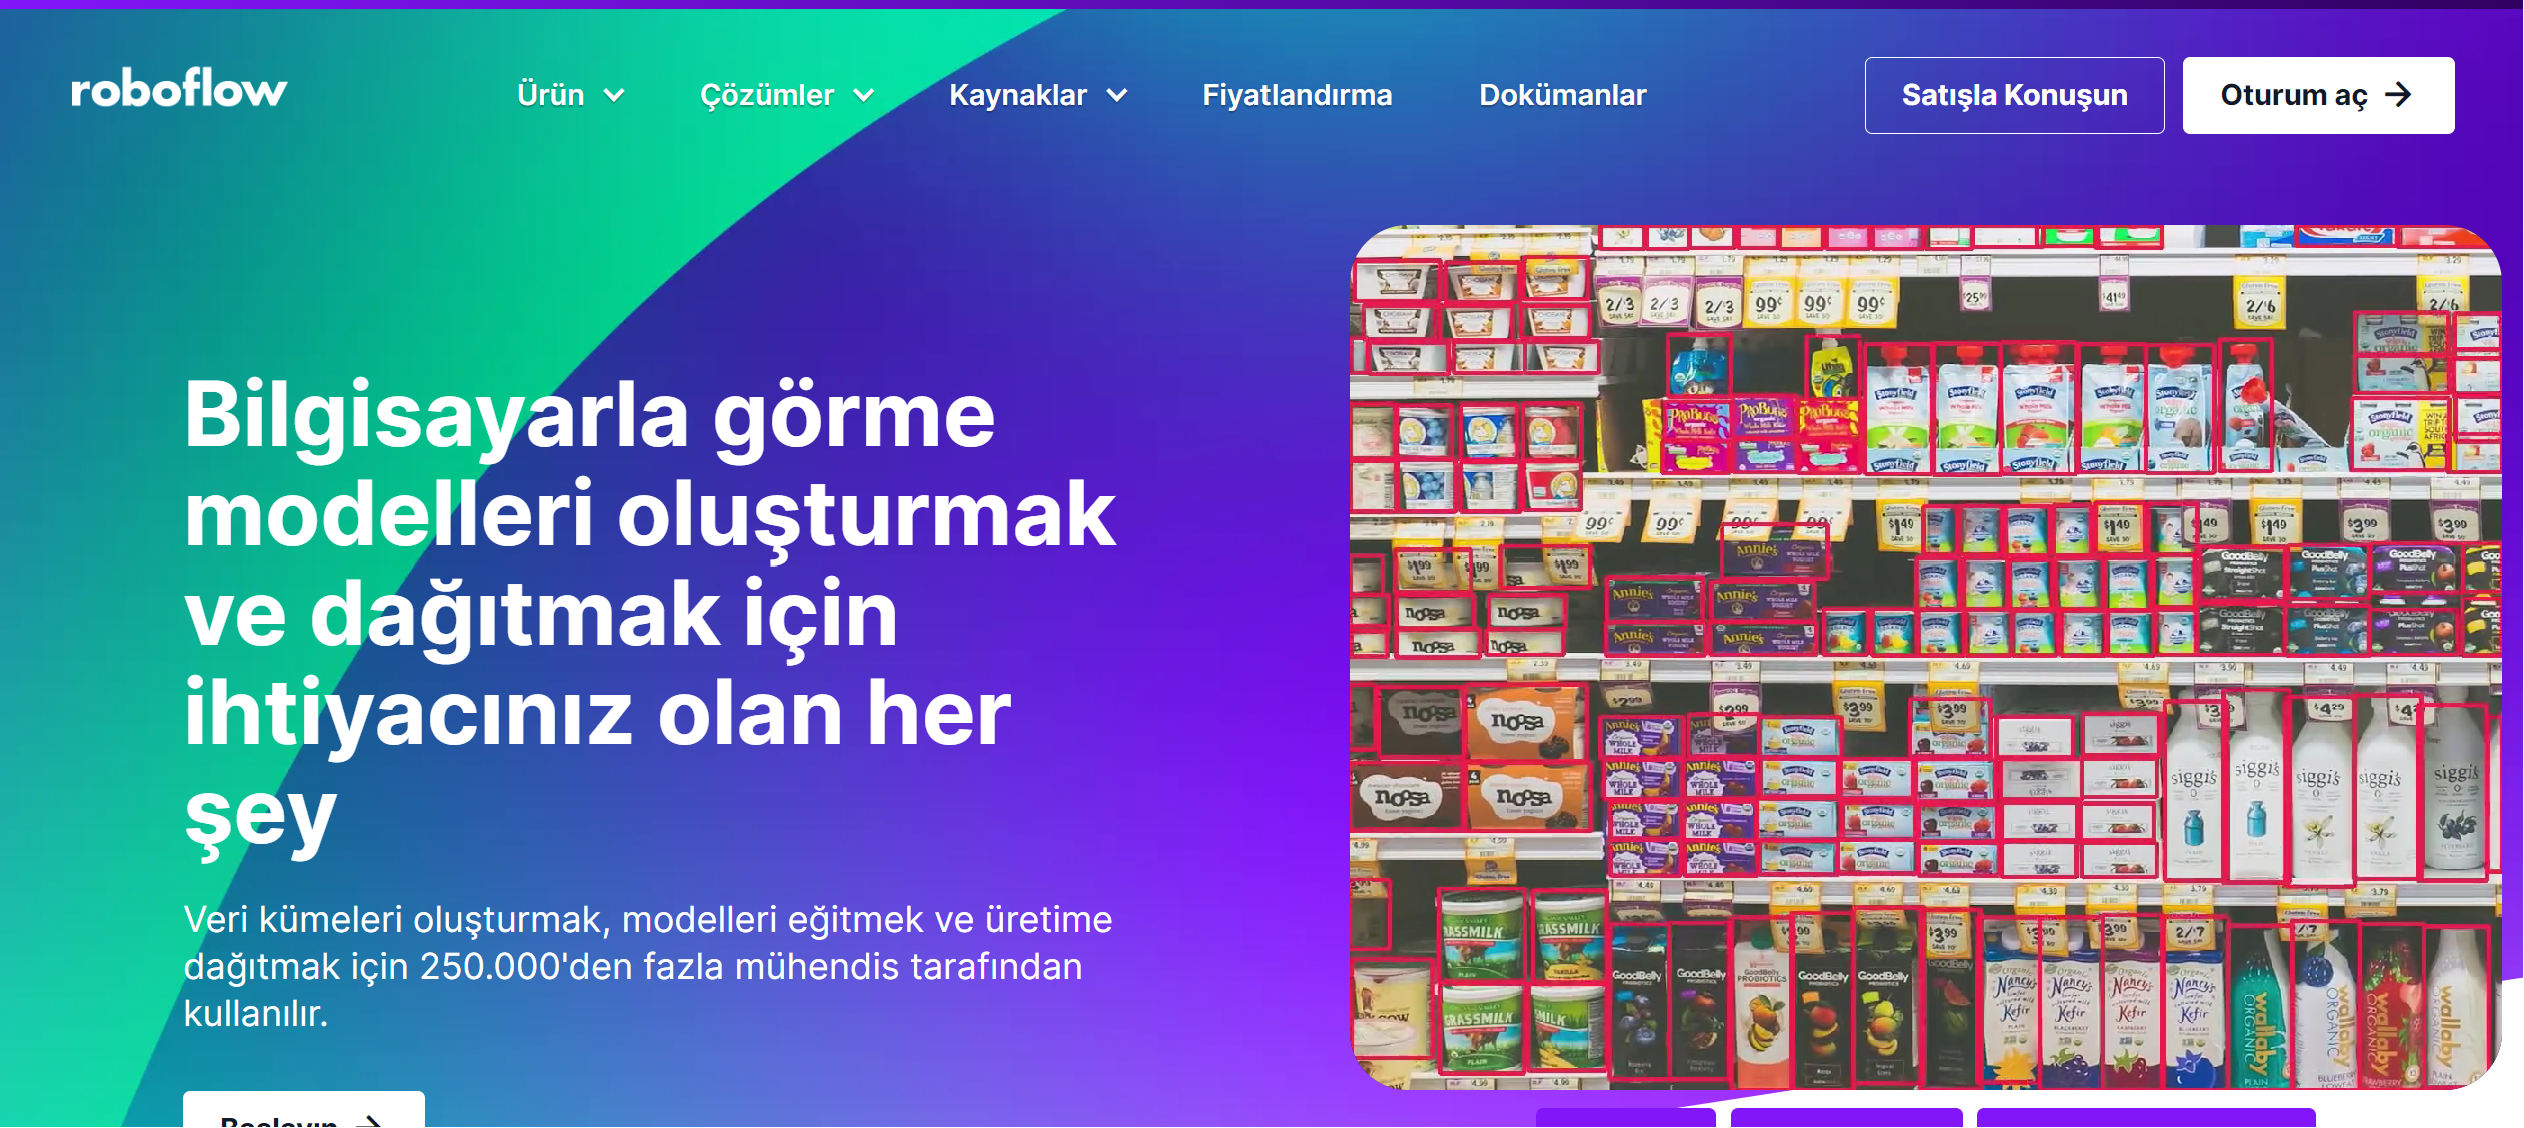
\includegraphics[ width=\textwidth]{roboflow.png}
    	\caption{Roboflow}
    \end{figure}
    \newpage
    
    Görüntü etiketleme, bilgisayarlı görü (Computer Vision) modellerinin geliştirilmesinde çok önemli bir adımdır. Görüntü etiketleme, görüntülerin bilgisayarlı görü algoritmaları tarafından daha kolay anlaşılmasını sağlamak için bir görüntüye ilgili bilgilerin eklenmesidir. Etiketleme aşamasında sınırlayıcı kutular ve hatta görüntüdeki farklı nesnelerin ayrıntılı segmentasyonları yer alabilir\cite{Ddataguess}.
    \newline
    
    \begin{figure}[!h]
    	\centering
    	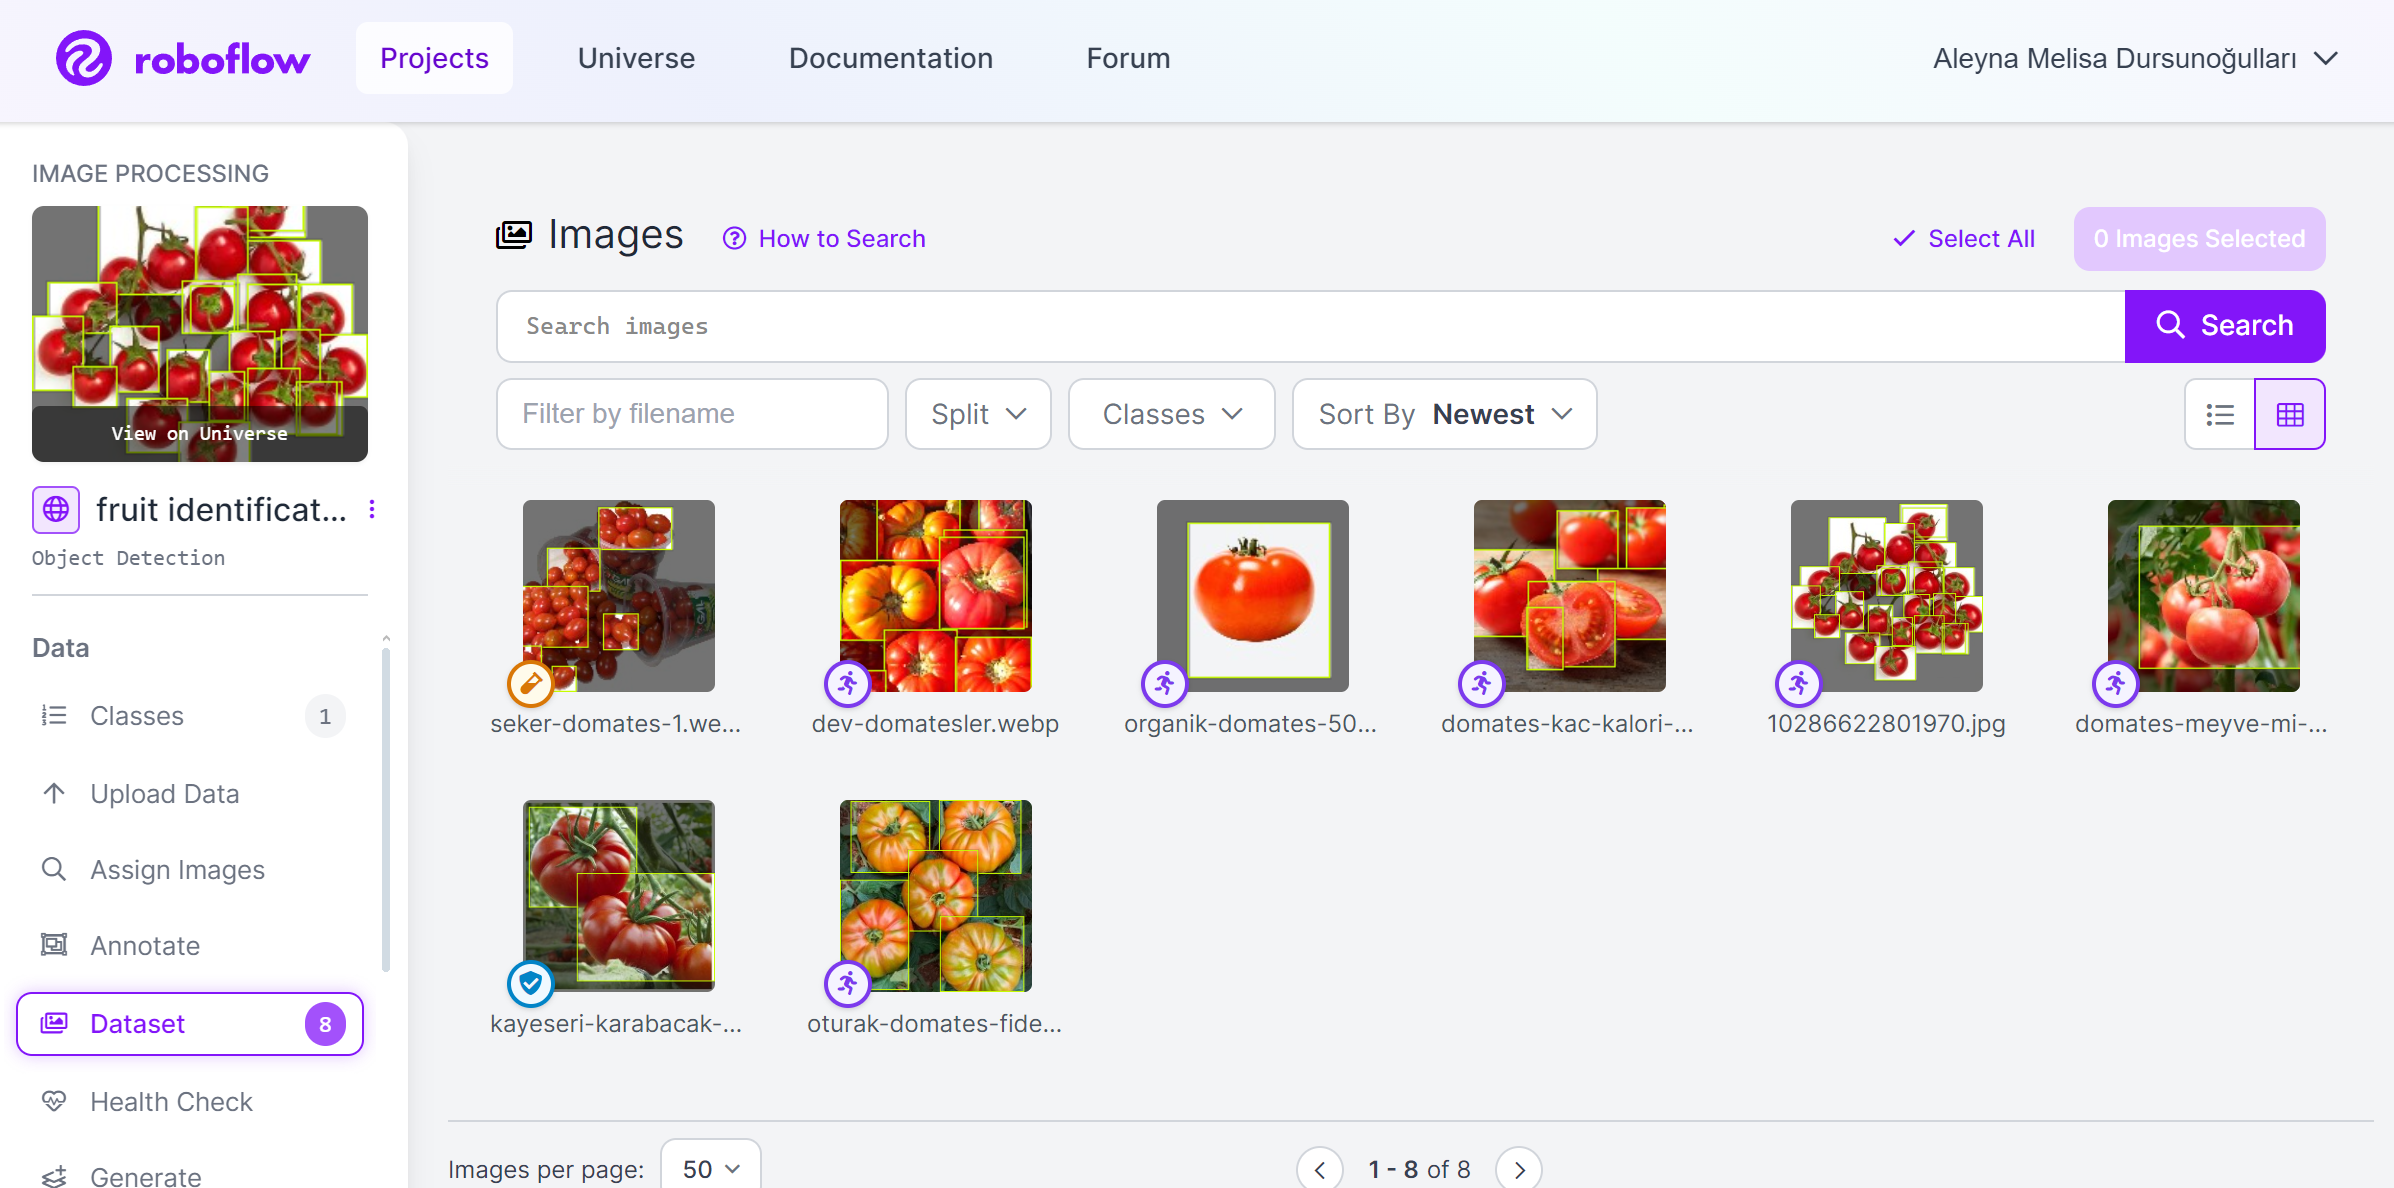
\includegraphics[ width=\textwidth]{etiketleme.png}
    	\caption{Roboflow : Etiketlemeye örnek}
    	
    	
    \end{figure}
    
    \begin{figure}[!h]
    	\centering
    	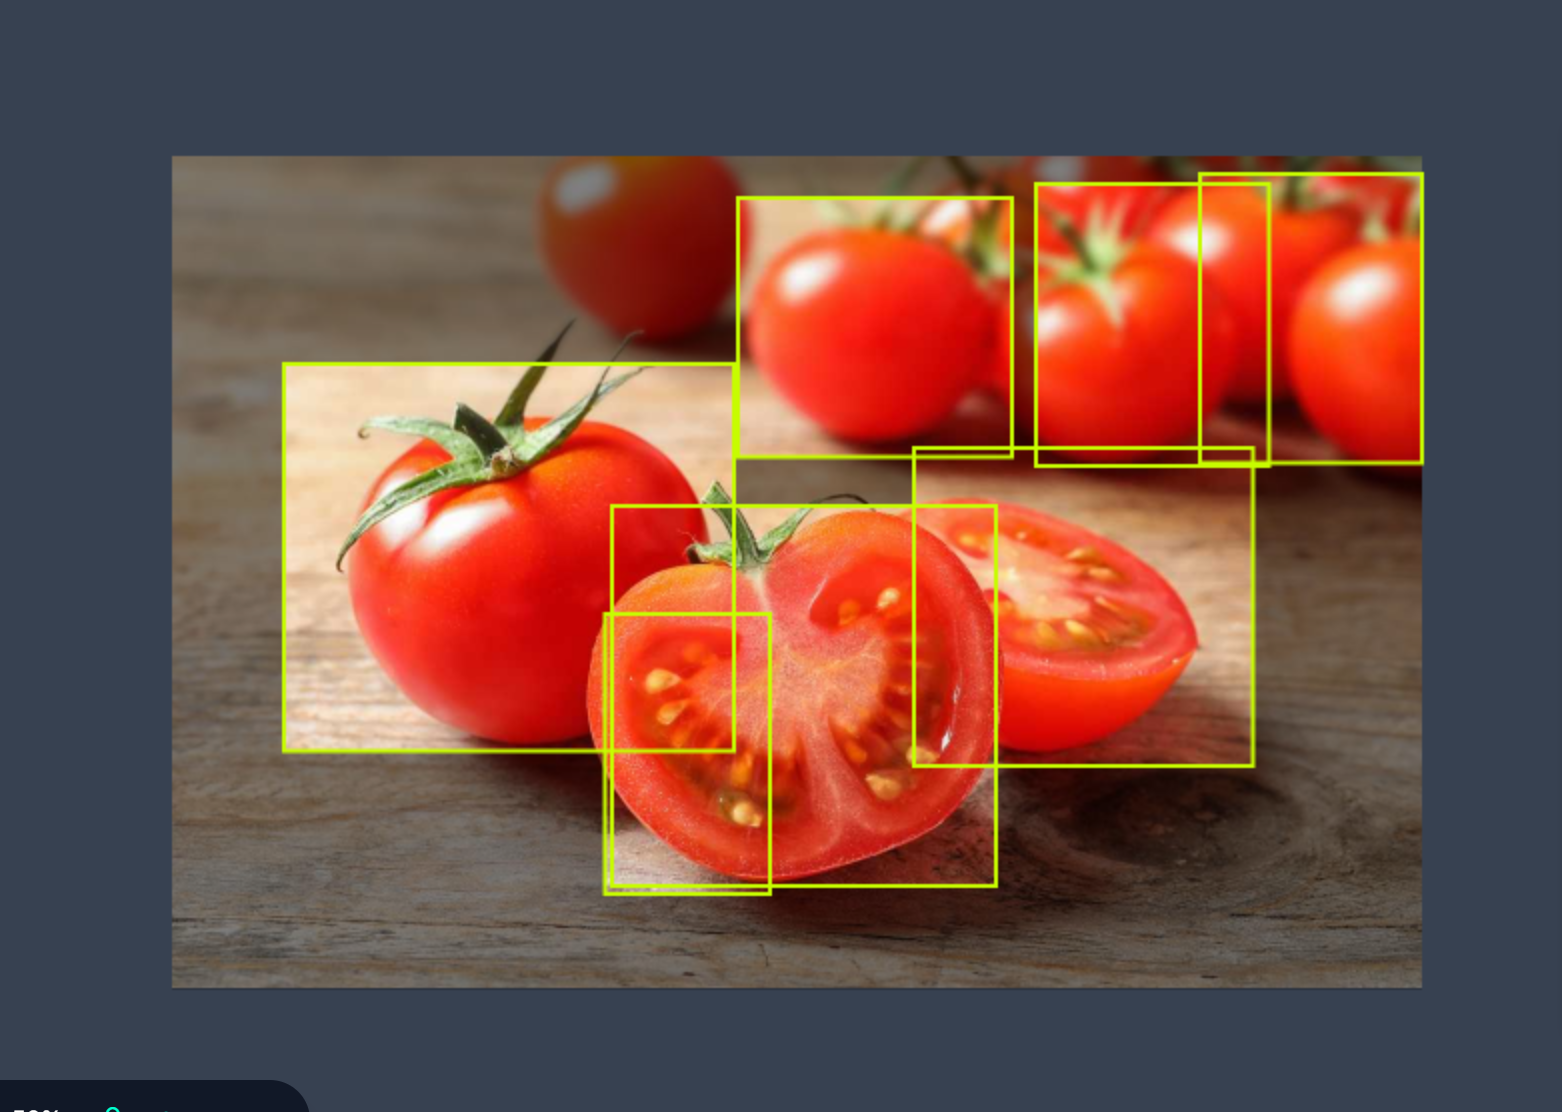
\includegraphics[ width=\textwidth]{etiket_ornek.png}
    	\label{ornek}
    	\caption{Roboflow}
    \end{figure}
    Şekil \ref{etiket} de etiketleme işlemine örnek verilmiştir.
    
    \newpage
    
    	YOLOv9,bilgisayarlı görme modelidir. Yolo v9 tanımlayıcı metinlere dayalı olarak bir görüntü içindeki herhangi bir nesnenin tespit edilmesini sağlar.YOLO serisi gerçek zamanlı nesne dedektörlerinin en son yinelemesidir ve doğruluk ve hız açısından en üst düzeyde performans sunar.Toplanan veriler etiketleme aşamasından sonra yolo v9 kullanılarak verilen veriler dışındaki nesneleride algılanması için eğitilir\cite{yolov9}.
    
    
    \begin{figure}[!h]
    	\centering
    	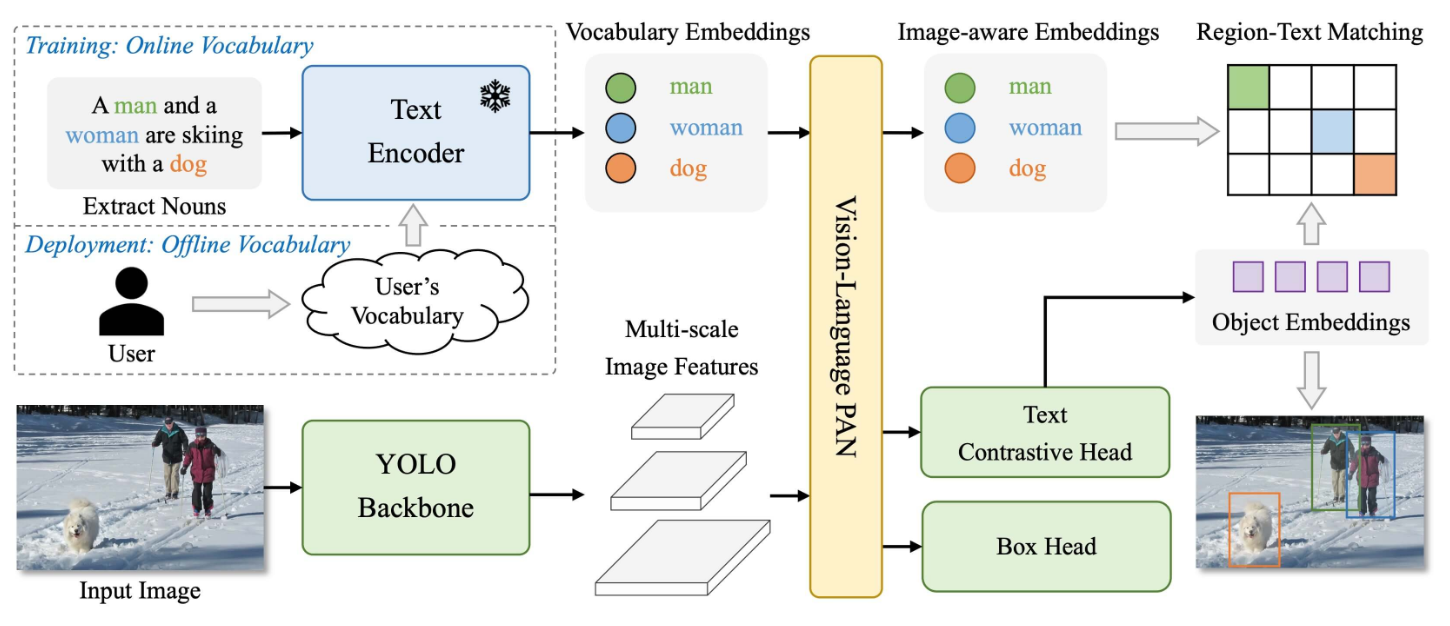
\includegraphics[ width=\textwidth]{yolo.png}
    	\caption{Yolov9}
    	
    \end{figure}
    \newpage
    Bu projede, görüntü işleme ve nesne tanıma alanında etkili bir derin öğrenme modeli olan CNN (Convolutional Neural Network) kullanılacaktır. CNN'ler, karmaşık görüntü verilerini işlemek, özelliklerini çıkarmak ve doğru bir şekilde sınıflandırmak için tasarlanmıştır. Bu model, veri setindeki nesnelerin ve özelliklerin tanınması ve sınıflandırılması sürecinde kullanılacak. CNN mimarileri, özellikle ImageNet gibi büyük veri setlerinde yüksek doğruluk elde etmek için başarıyla kullanılmıştır. Bu projede de CNN modeli, görüntülerin anlamını ve içeriğini analiz etmek için temel bir araç olacaktır.
   \newline
    
    OpenCV (Open Source Computer Vision) açık kaynak kodlu görüntü işleme kütüphanesidir.OpenCV kütüphanesi içerisinde görüntü işlemeye (image processing) ve makine öğrenmesine (machine
    learning) yönelik 2500’den fazla algoritma bulunmaktadır. Bu algoritmalar ile yüz tanıma, nesneleri ayırt etme, insan hareketlerini tespit edebilme, nesne sınıflandırma, plaka tanıma, üç boyutlu görüntü üzerinde işlem yapabilme, görüntü karşılaştırma, optik karakter tanımlama OCR (Optical Character Recognition) gibi işlemler rahatlıkla yapılabilmektedir. Etiketlenen verilerdeki nesneleri etiket yardımı ile tanımlamayı sağlar.Görüntüleri anlamlandırmak için geniş bir araç seti sunar\cite{opencv}.
	\newline
	
	\begin{figure}[!h]
		\centering
		
\includegraphics[width=0.25\textwidth]{OpenCV.png}
		\label{etiket}
		\caption{OpenCV}
		
	\end{figure}
    \newpage
     TensorFlow, açık kaynak kodlarını içerisinde barındıran derin öğrenme (Deep Learning) kütüphanesi olarak ifade edilebilir. TensorFlow’un esnek yapısı, tek API (Application Programming Interface), uygulama programlama arayüzü ile tüm platformlarda hesapların yapılmasını sağlamaktadır. Tanımlaması yapılan yiyeceklerin boyutuda göz önüne alınırak tensorflow kütüphanesi ile kalori hesaplaması yapılacaktır\cite{Tensorflow}.
     \newline
     
     \begin{figure}[!h]
     	\centering
     	
\includegraphics[ width=\textwidth]{Tensorflow.png}
     	\caption{TensorFlow}
     	
     \end{figure}
     
     
     	\item[\textbf{3.2}]\textbf{KULLANILABİLİCEK KÜTÜPHANELER}
     	 \begin{itemize}
     		\item OpenCV
     		\item TensorFlow
     		\item Keras
     		\item YOLO (You Only Look Once)
     		\item PyTorch
     		\item Scikit-Image (skimage)
     		\item Faster R-CNN (Region-based Convolutional Neural Networks)
     		\item Caffe
     		
     		
     	\end{itemize}
     	
     	 \begin{landscape}
     		\begin{figure}[!h]
     			
     			\raggedright
     			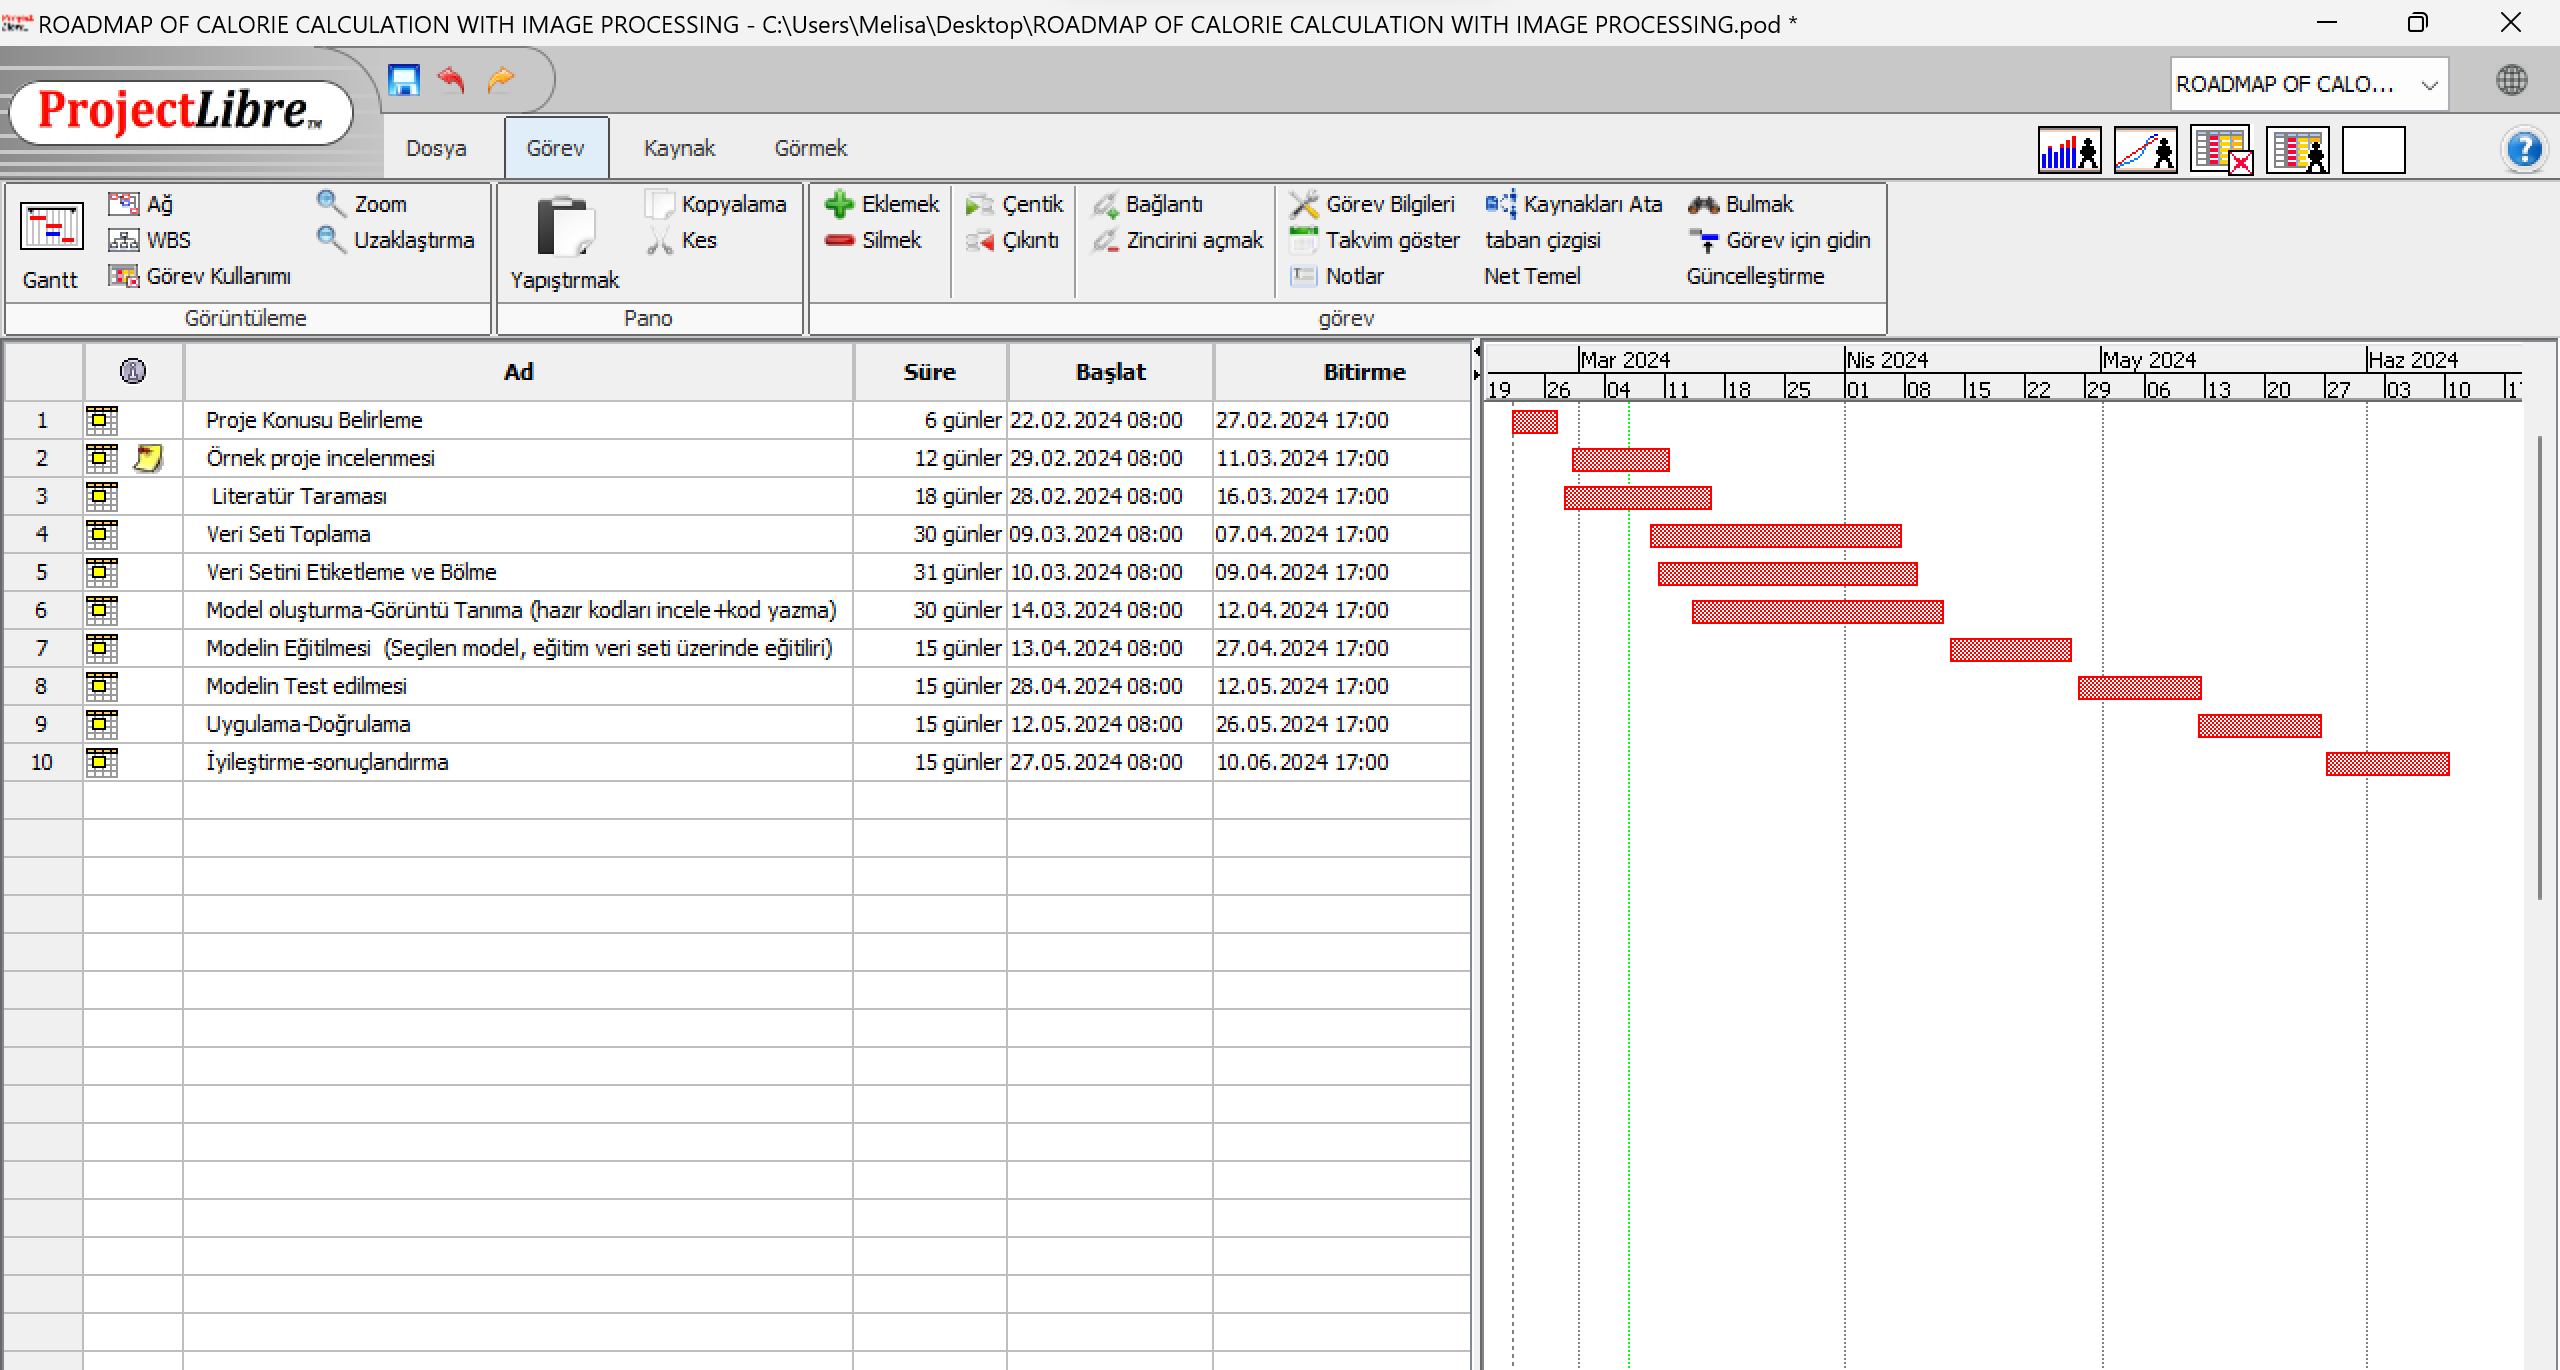
\includegraphics[height=1.04\textheight]{Roadmap}
     			\caption{İş Planı}
     			
     		\end{figure}
     	\end{landscape}
     	
     	\begin{landscape}
     		\begin{figure}[!h]
     			
     			\raggedright
     			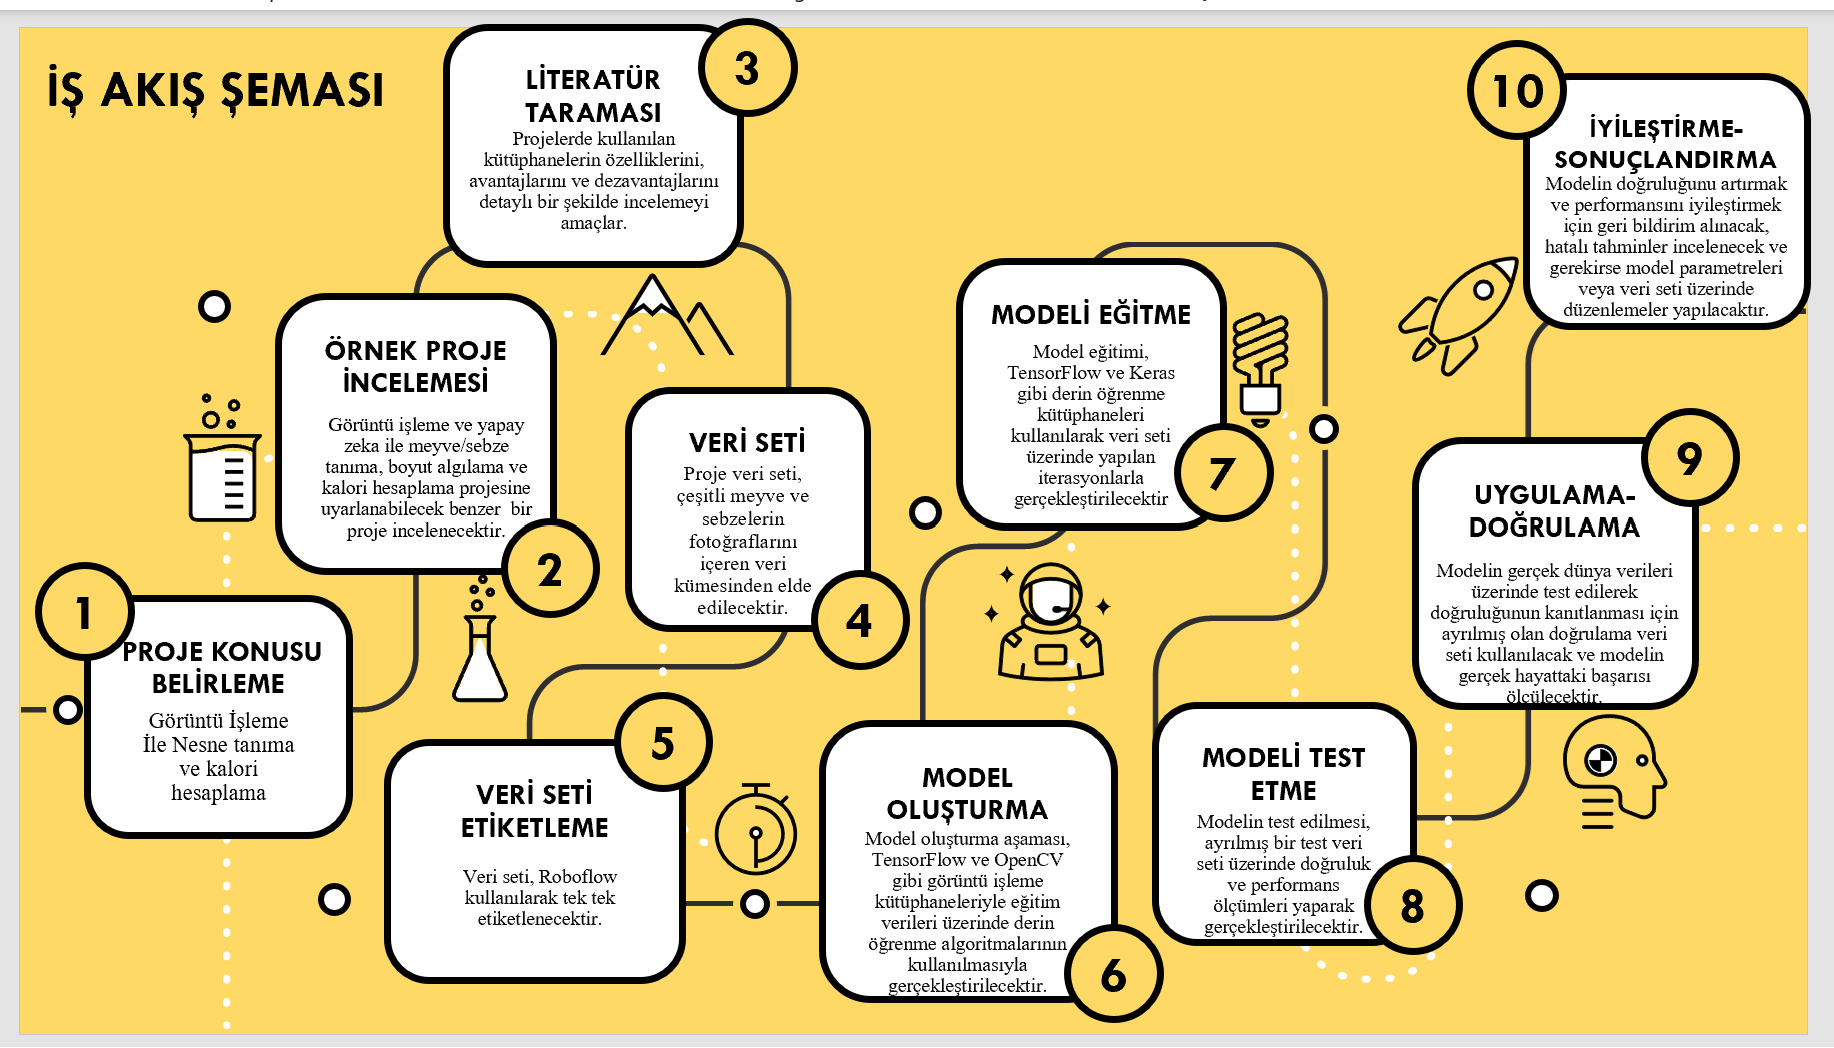
\includegraphics[height=1.04\textheight]{İş Akış Şeması}
     			\caption{İş Akış Şeması}
     			
     		\end{figure}
     	\end{landscape}
    \end{enumerate}
    \newpage
    
	\section{Veritabanı Ve Veriler}
	
	\begin{figure}[!h]
		
		\centering
		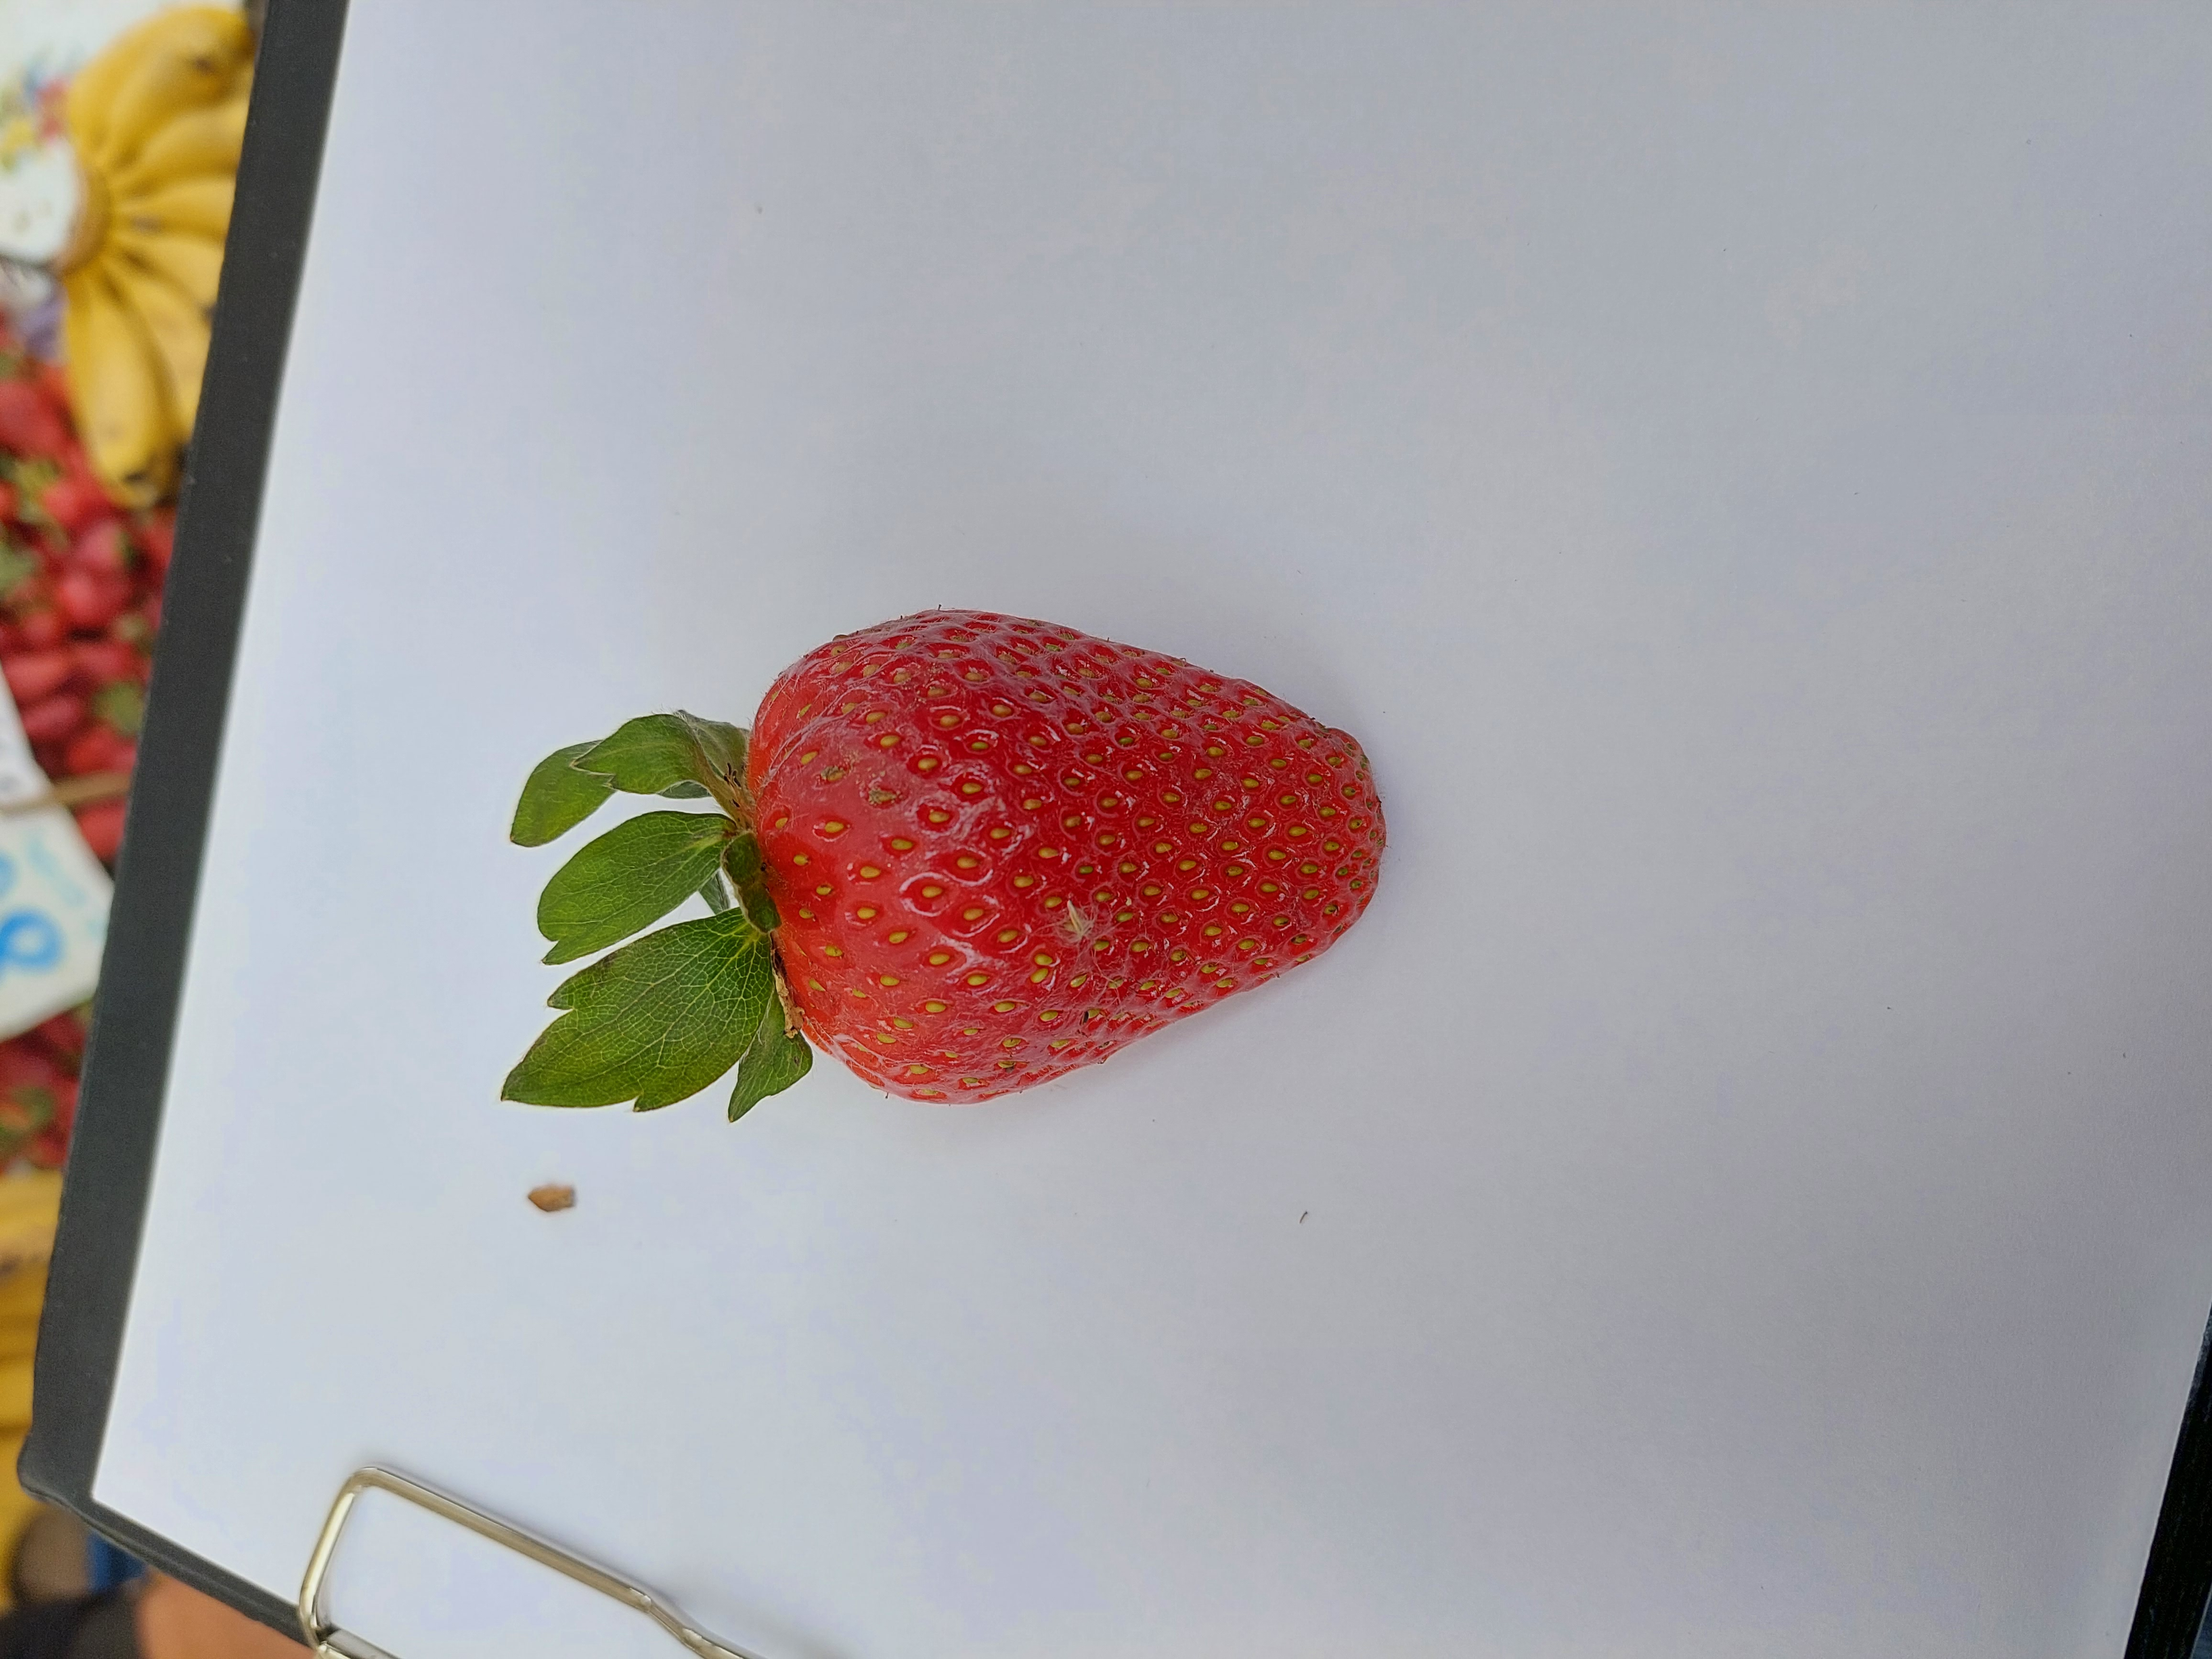
\includegraphics[angle=-90,width=0.5\textwidth]{resim1}
		\caption{Veri Örneği-1}
		
	\end{figure}
	
	
	\begin{figure}[!h]
		
		\centering
		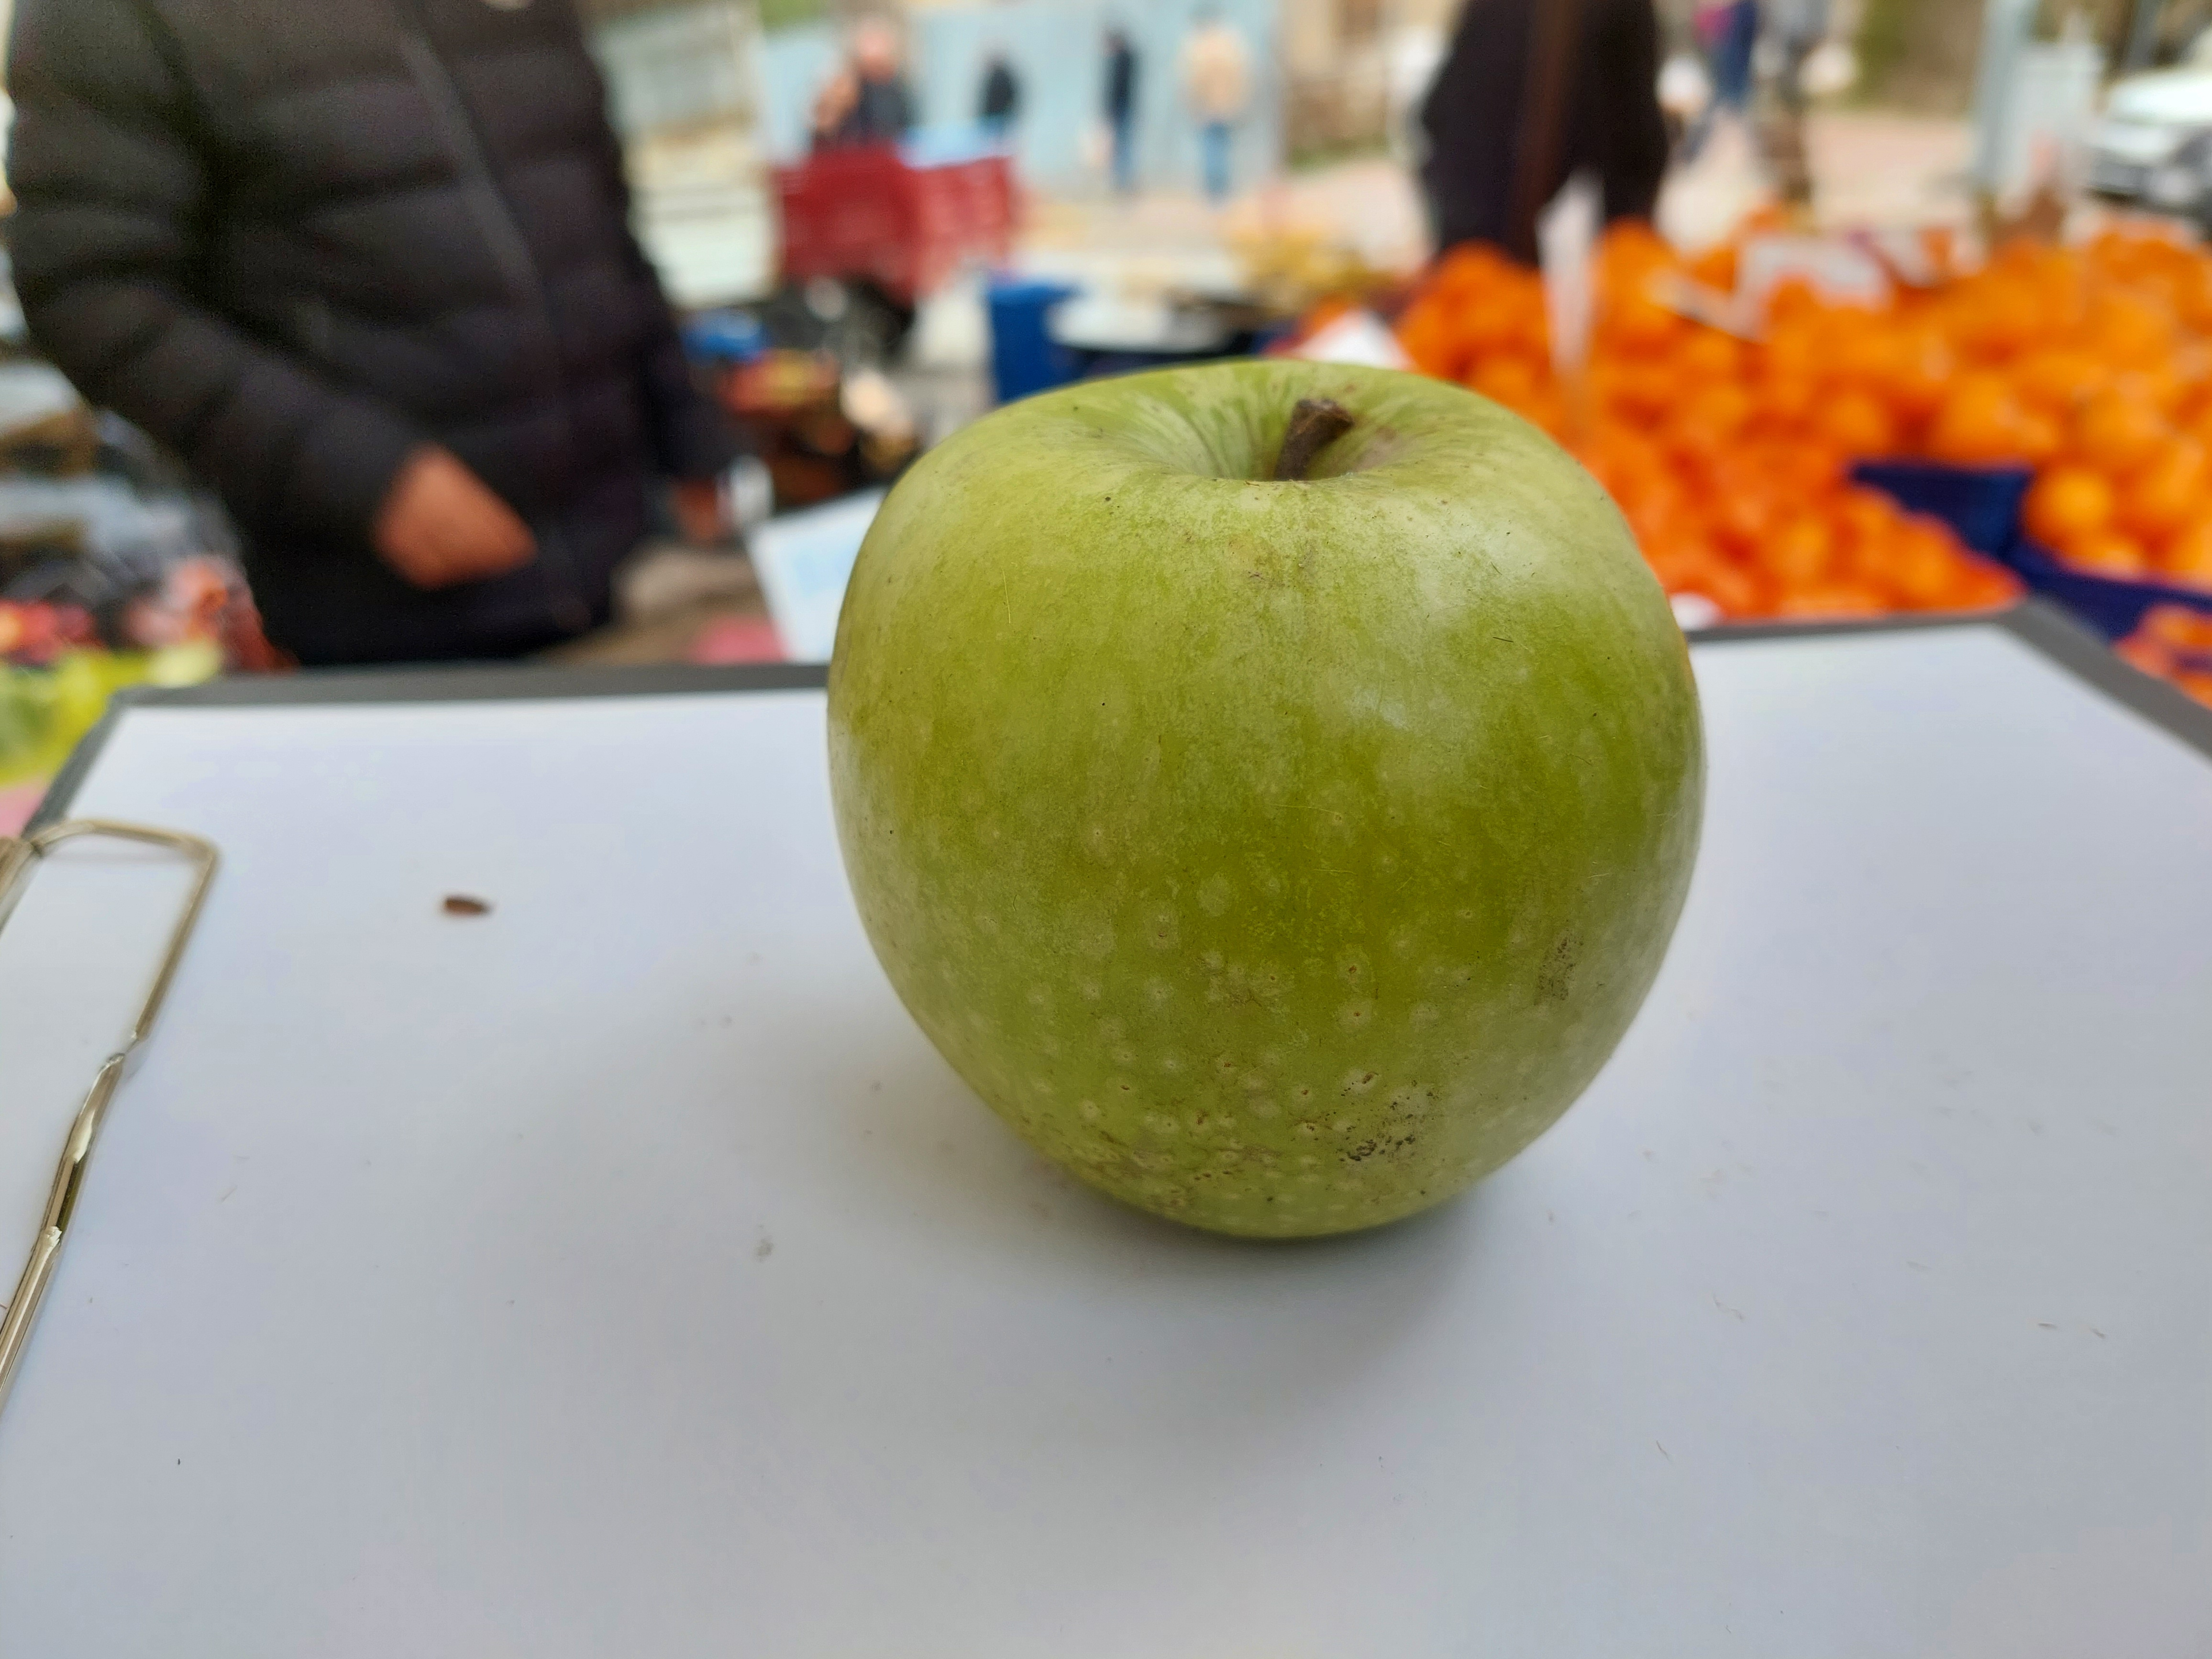
\includegraphics[width=0.5\textwidth]{resim2}
		\caption{Veri Örneği-2}
		
	\end{figure}
	
	\begin{figure}[!h]
		
		\centering
		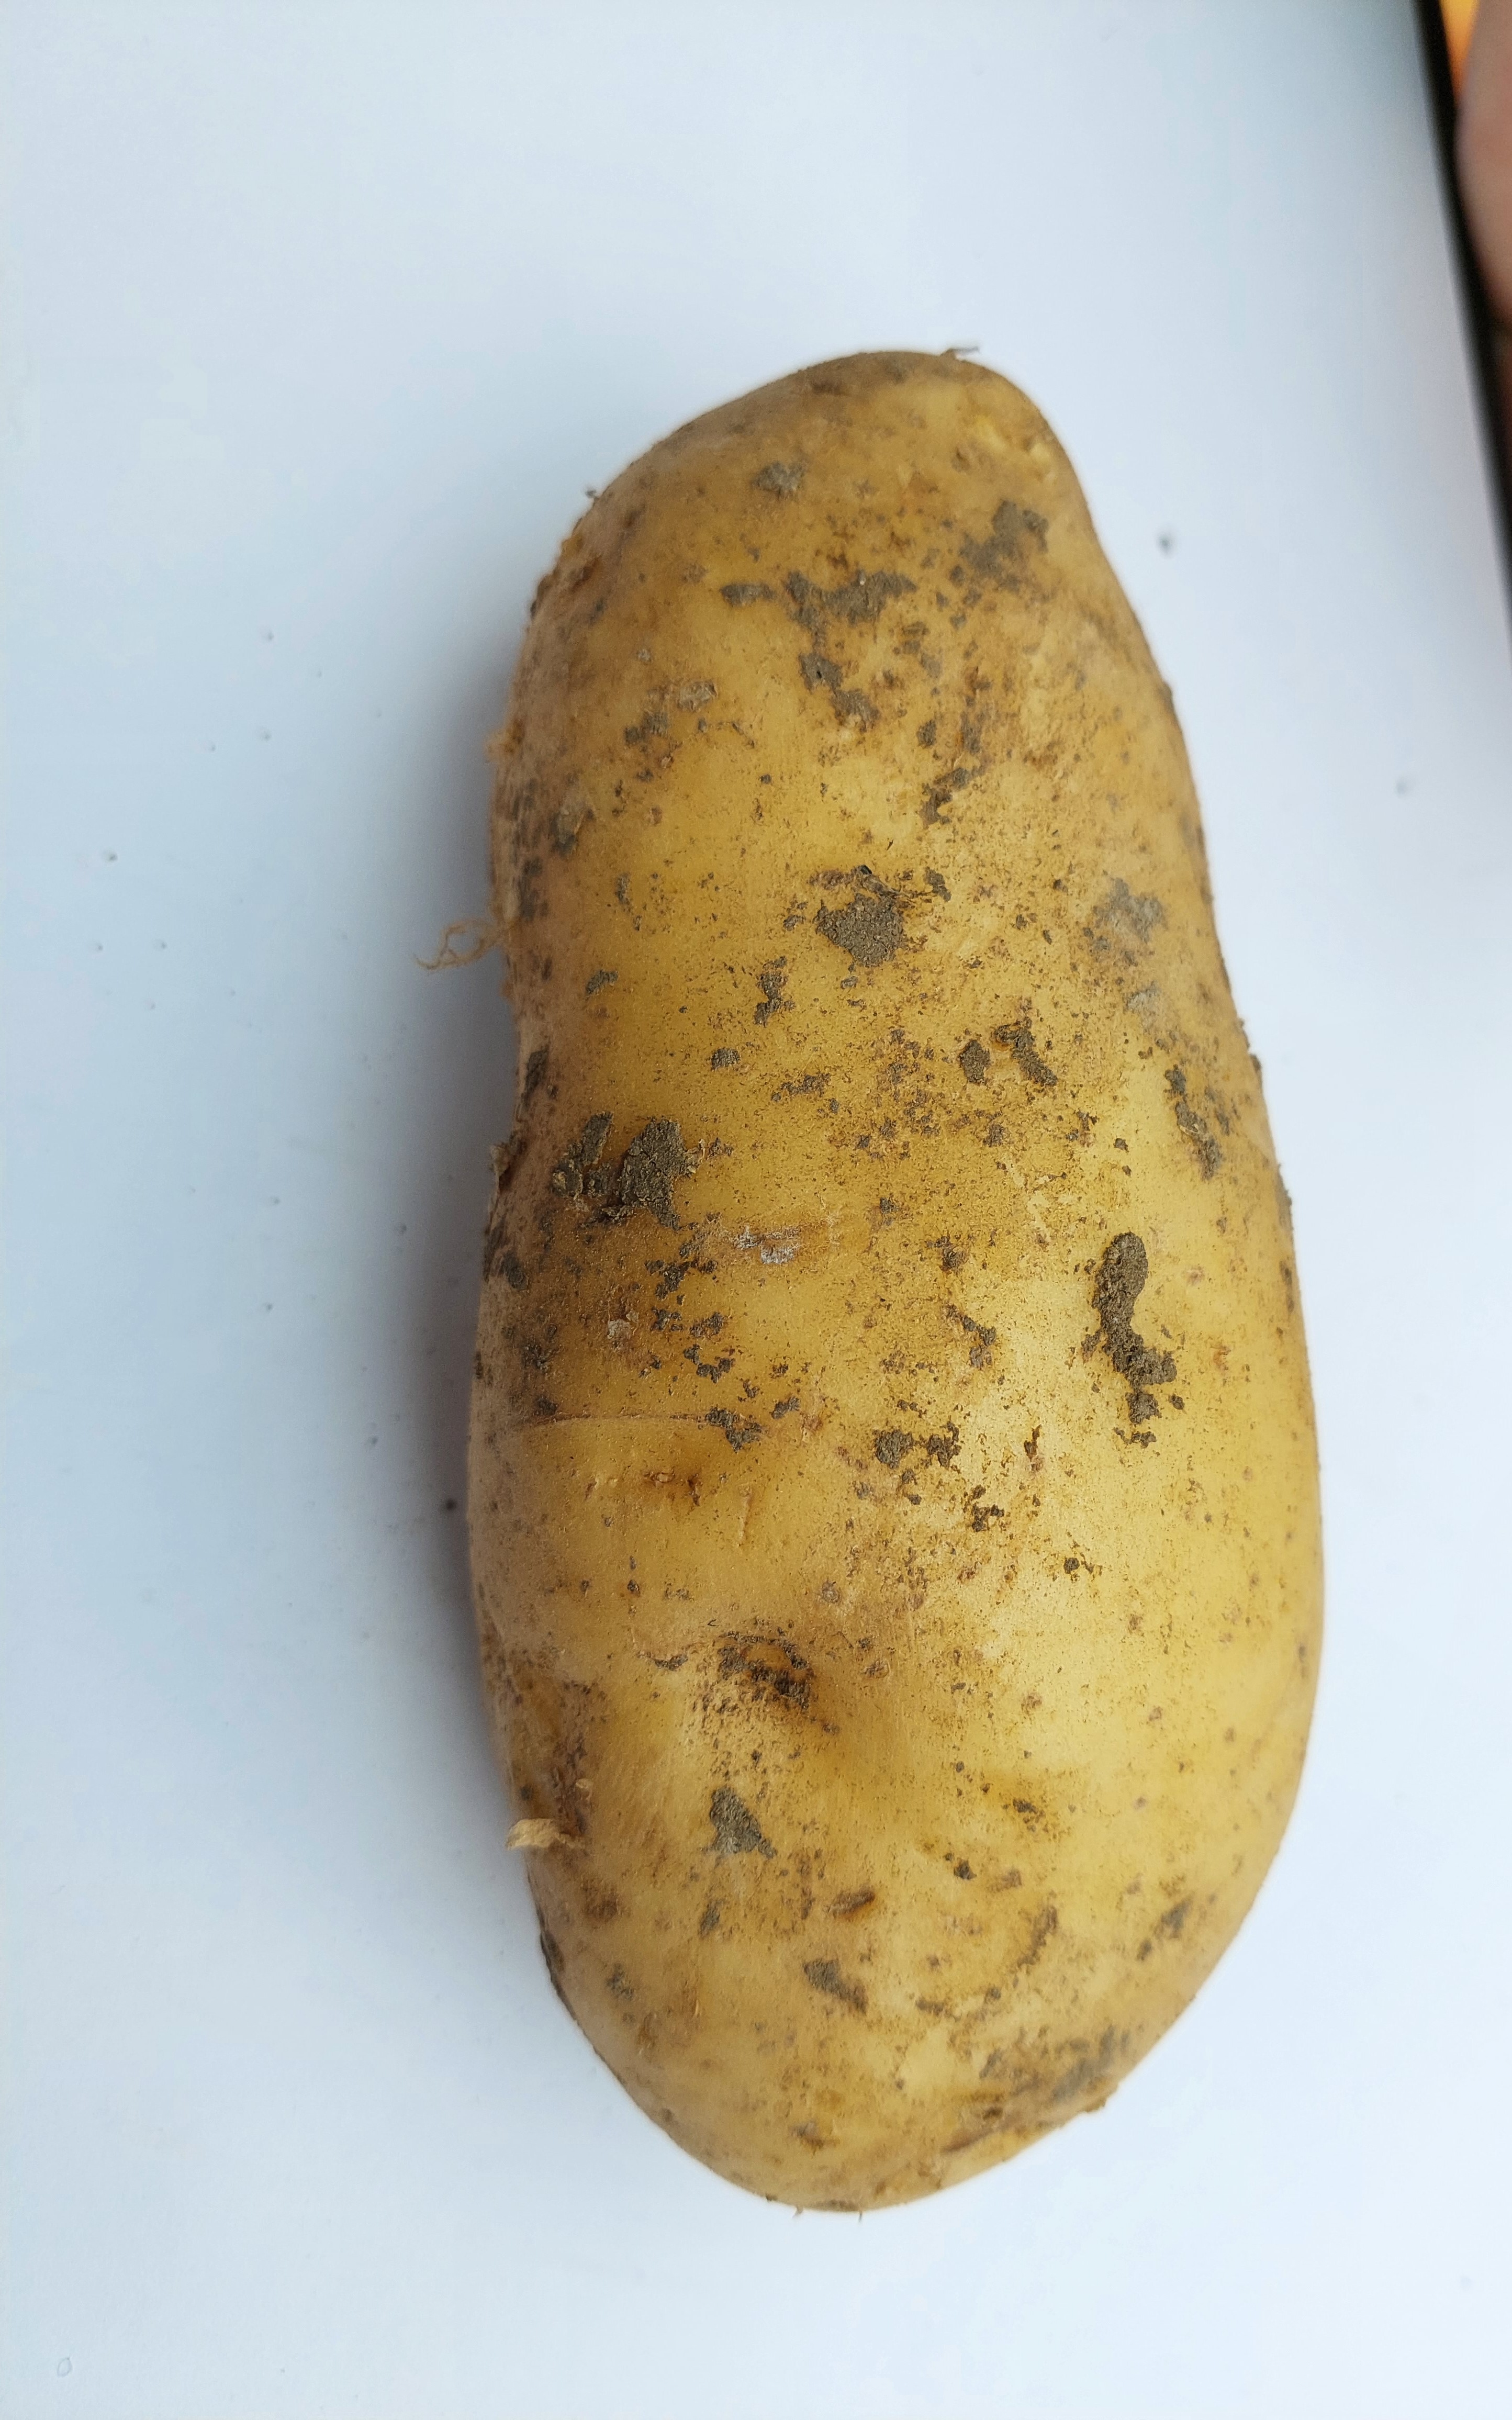
\includegraphics[angle=90,width=0.5\textwidth]{resim3}
		\caption{Veri Örneği-3}
		
	\end{figure}
	
	\begin{figure}[!h]
		
		\centering
		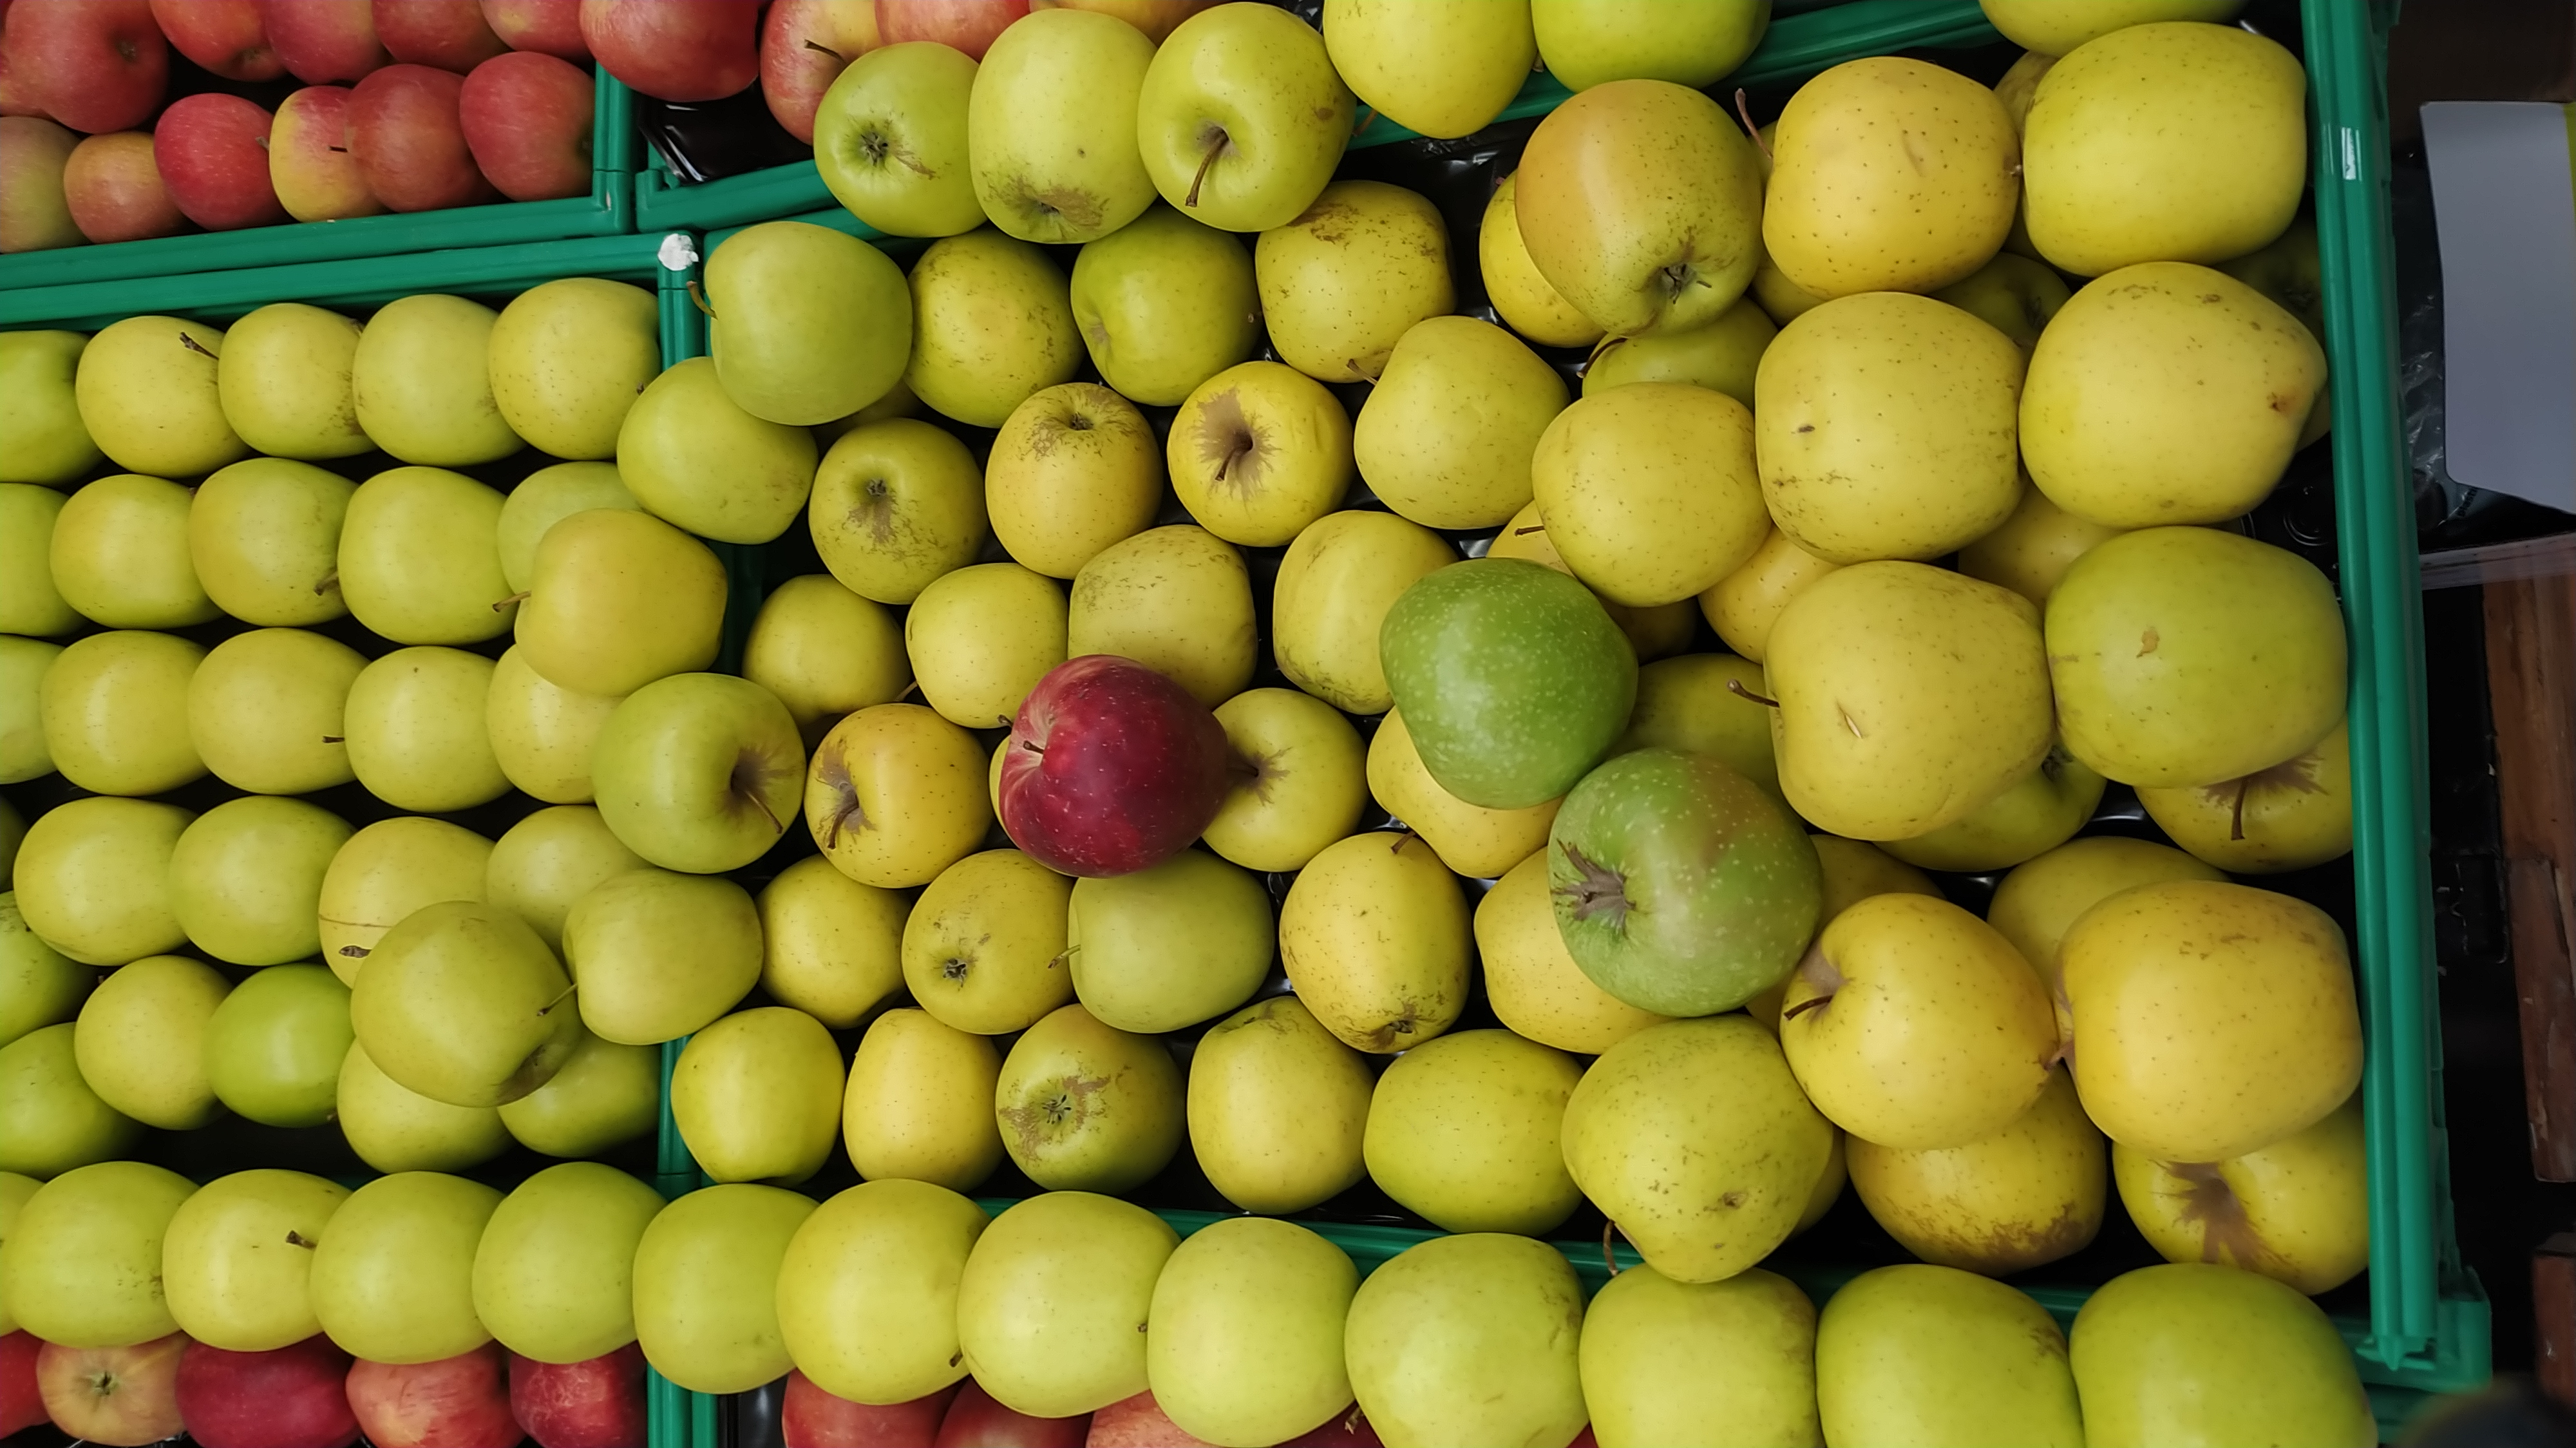
\includegraphics[angle=-90,width=0.5\textwidth]{resim4}
		\caption{Veri Örneği-4}
		
	\end{figure}
	\newpage
	\begin{figure}[!h]
		
		\centering
		\includegraphics[width=0.5\textwidth]{resim5}
		\caption{Veri Örneği-5}
		
	\end{figure}
	
	\begin{figure}[!h]
		
		\centering
		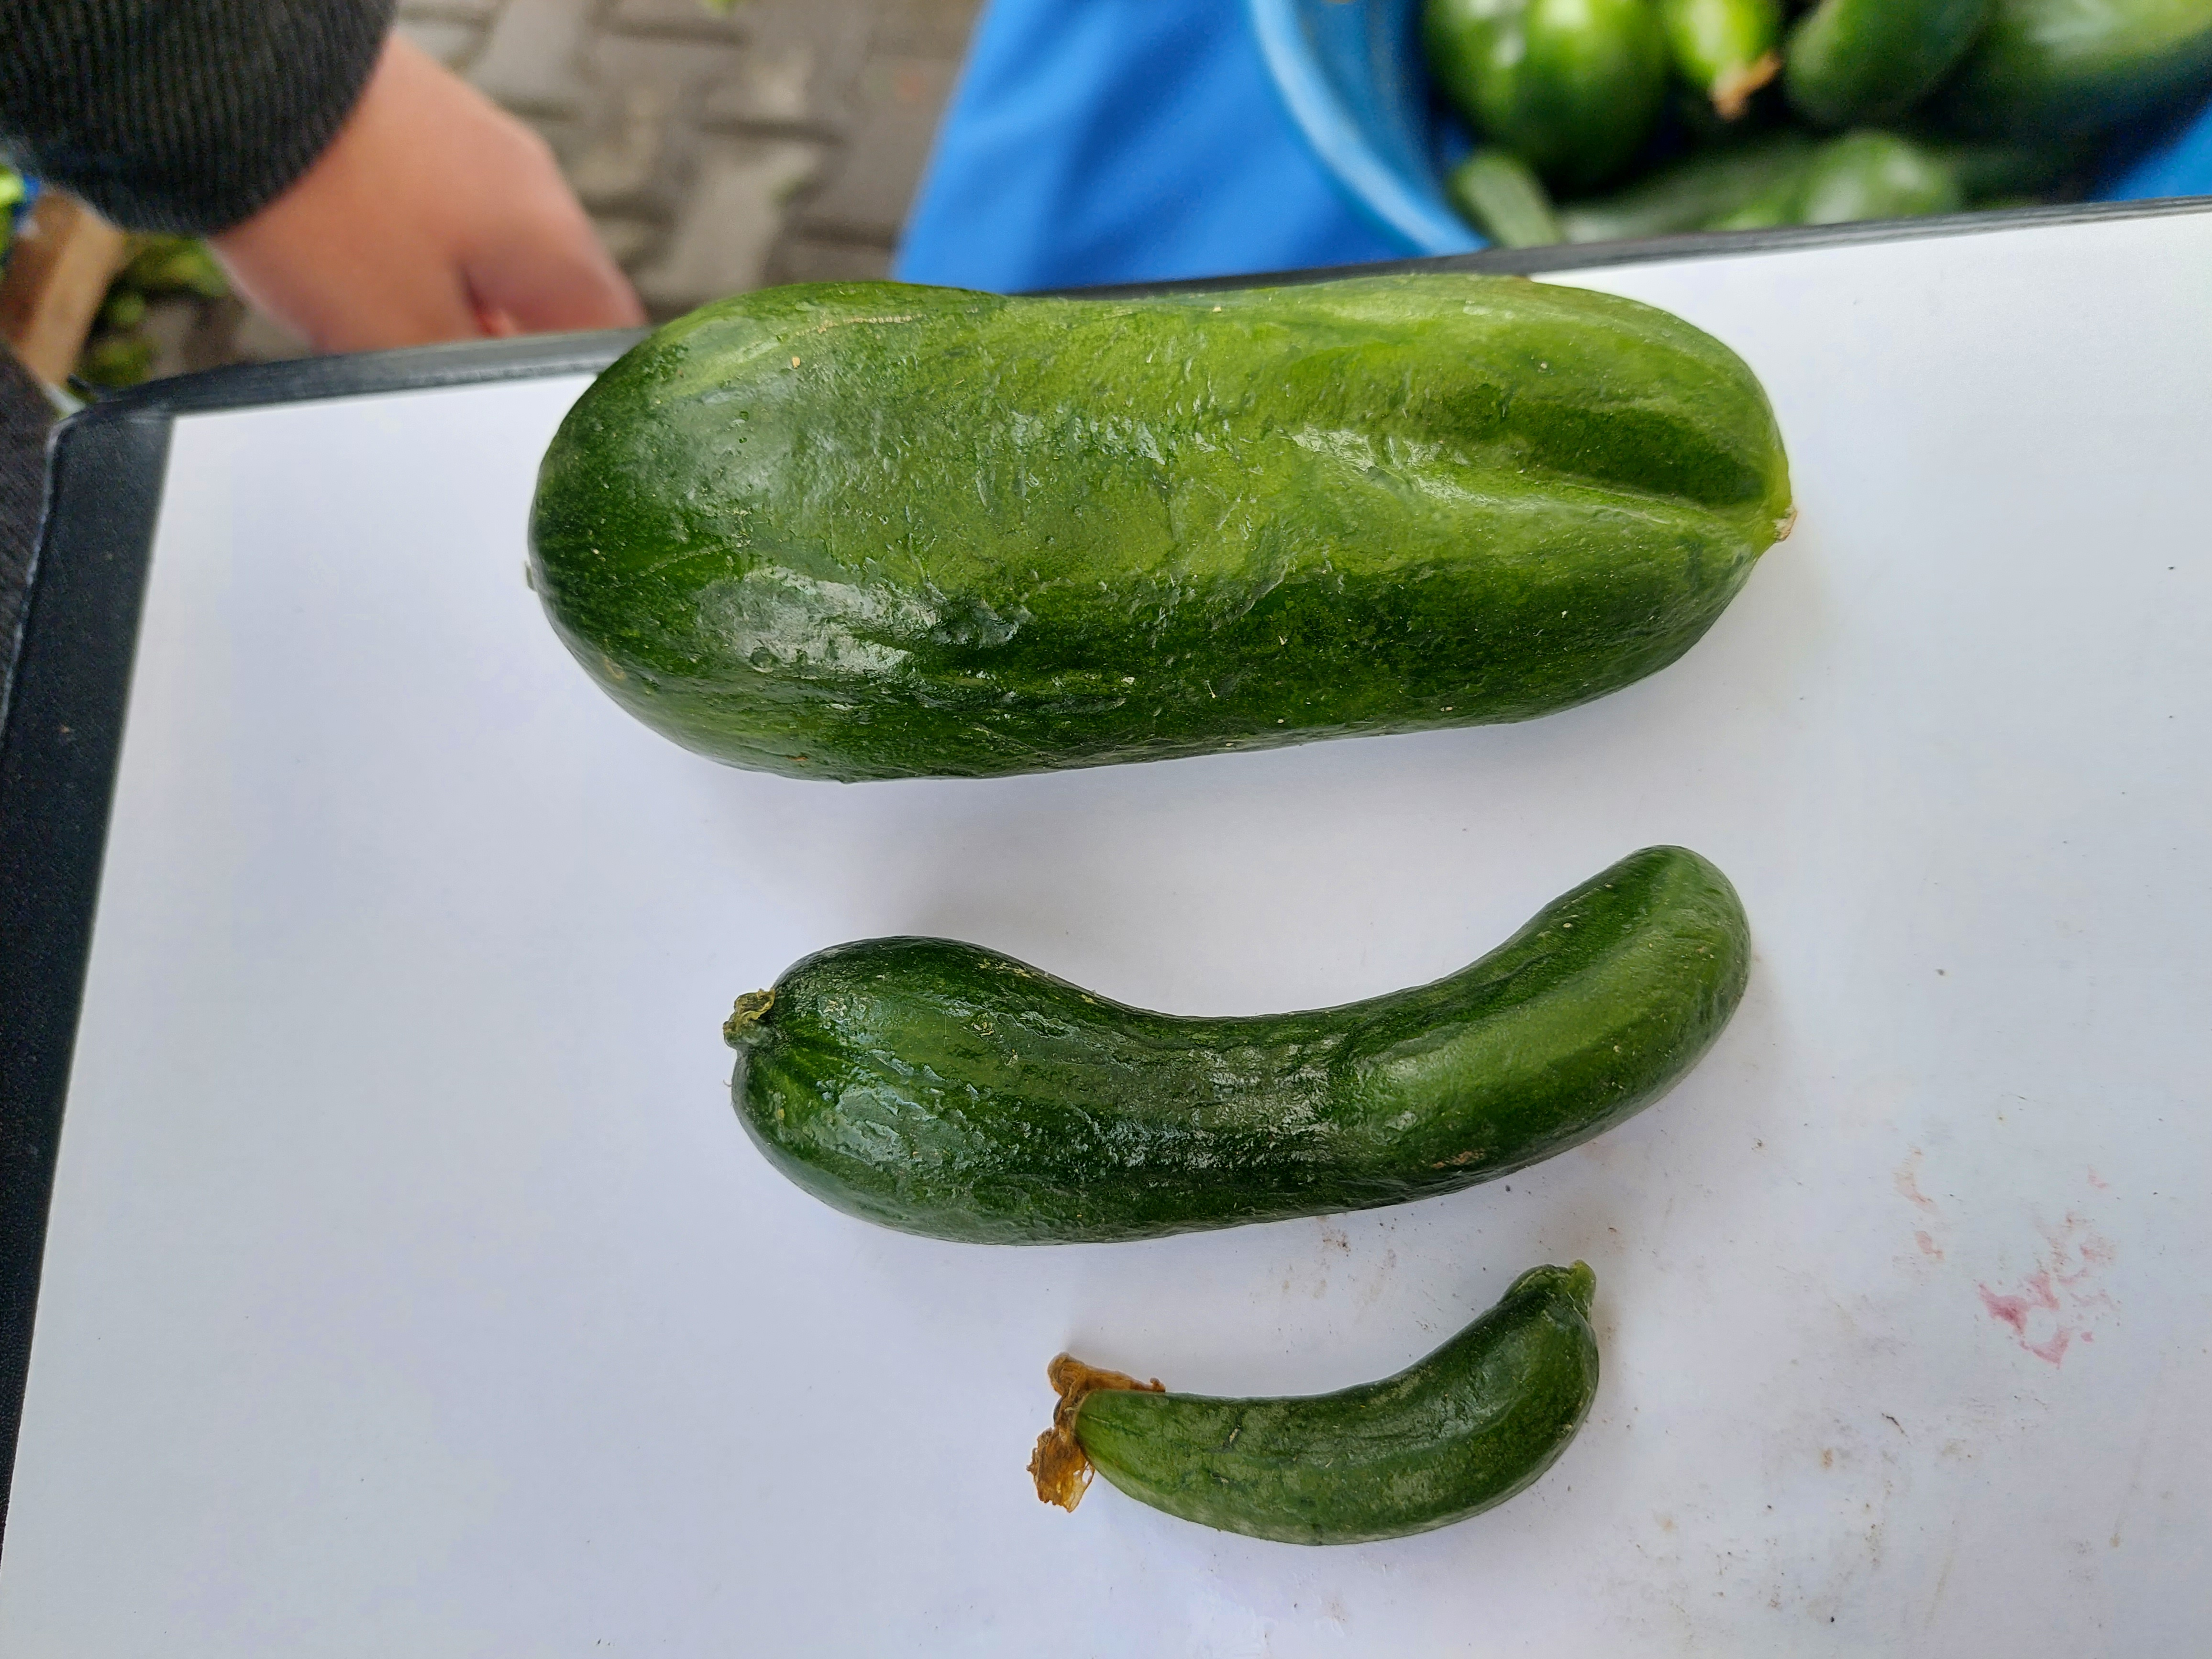
\includegraphics[angle=-90,width=0.5\textwidth]{resim6}
		\caption{Veri Örneği-6}
		
	\end{figure}
	
	\begin{figure}[!h]
		
		\centering
		\includegraphics[angle=-90,width=0.5\textwidth]{resim7}
		\caption{Veri Örneği-7}
		
	\end{figure}
	\begin{figure}[!h]
		
		\centering
		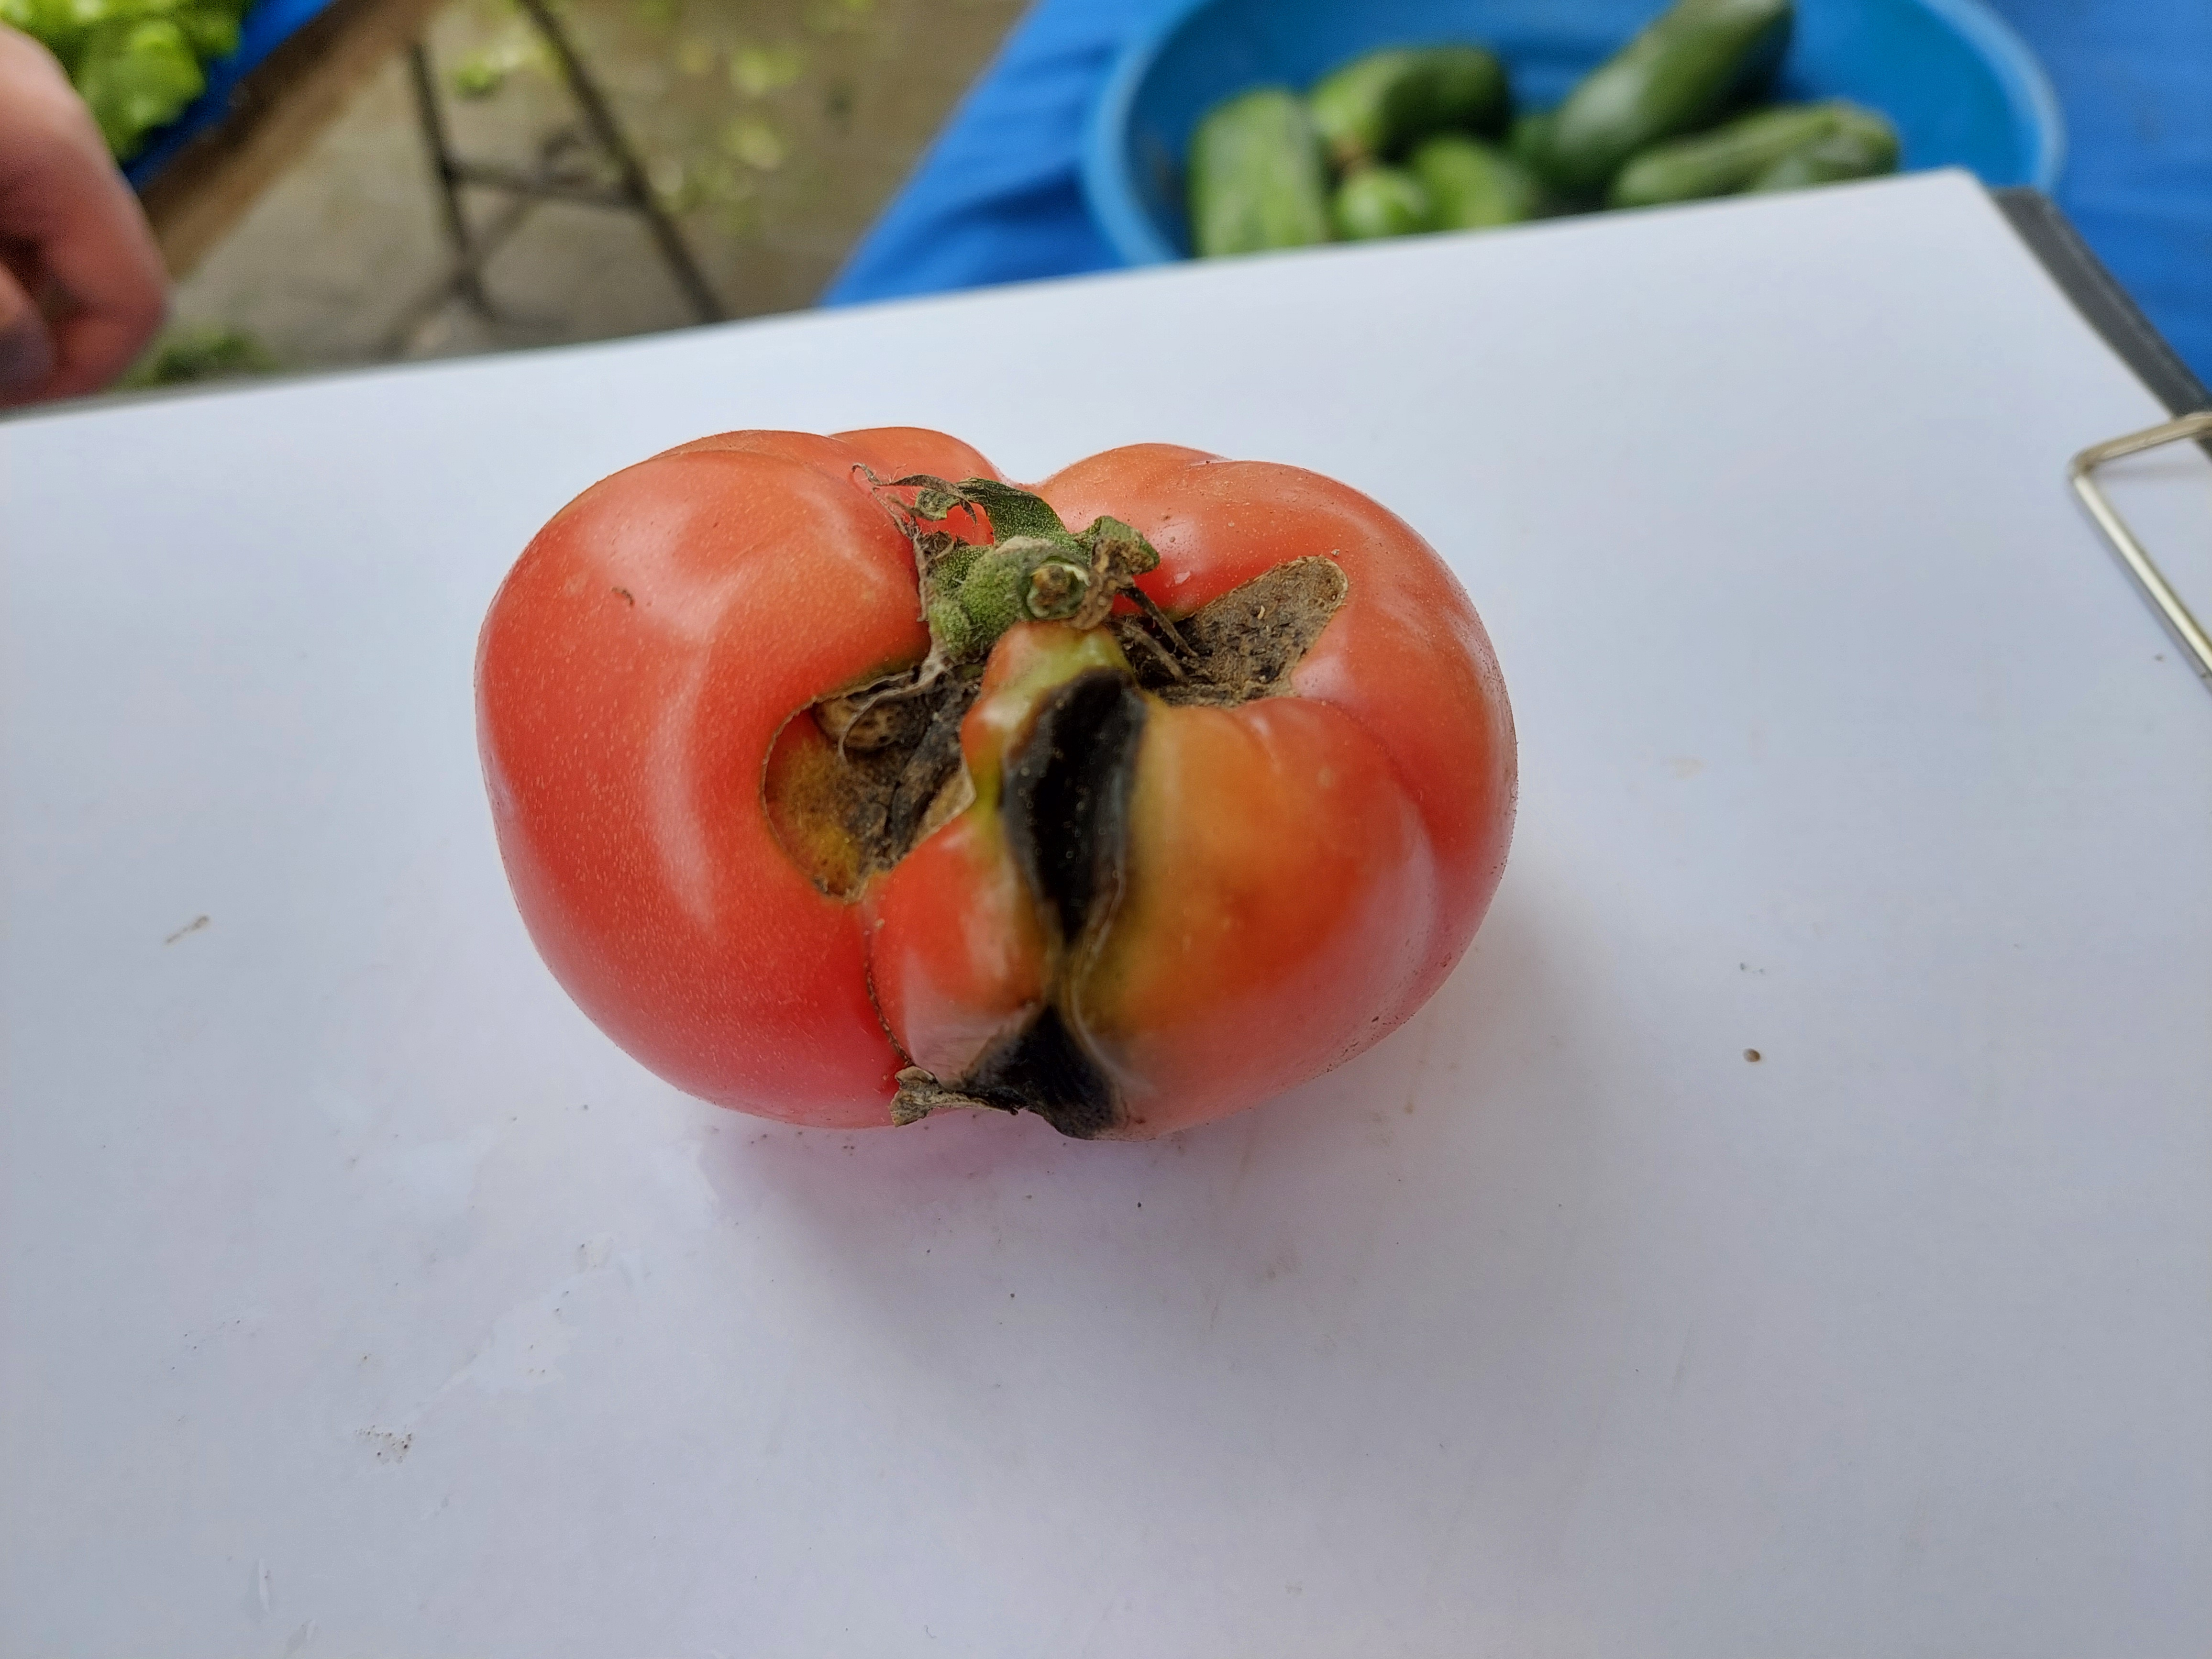
\includegraphics[width=\textwidth]{resim8}
		\caption{Veri Örneği-8}
		
		Projede kullanılacak veriler özel olarak toplanmıştır.Veri tabanında başlangıç olarak 600 veri bulunmaktadır. 
	\end{figure}
	
    \clearpage
    
    \section{Beklenen Sonuçlar}
     Bu projenin hedefi, fotoğraflardaki meyve ve sebzeleri tanıyarak, boyutunu algılayarak, kalori değerlerini hesaplayan ve çürük kısımları tespit eden bir yapay zeka modeli geliştirmektir. 
    \newline
    
    Aşağıda projenin beklenen sonuçları yer almaktadır:
    \newline
    
    \textbf{Meyve ve Sebzelerin Tanınması:} 
    \begin{itemize}
      \item Proje, geniş bir meyve ve sebze veri kümesi üzerinde eğitilecek ve çeşitli meyve ve sebzeleri doğru bir şekilde tanıyabilecektir.
      \item Örneğin, elma, muz, portakal gibi meyveleri ve domates, salatalık, patates gibi sebzeleri başarıyla tanıyabilecektir.
    \end{itemize}
  
    
    \textbf{Boyut Algılama:} 
    \begin{itemize}
      \item Fotoğraftaki meyve veya sebzenin boyutunu algılayarak, yaklaşık olarak gerçek boyutunu belirleyebilecektir.
      \item Örneğin, küçük, orta, büyük gibi boyutlar üzerinden bir tahmin yapabilecektir.
    \end{itemize}
    
    \textbf{Kalori Hesaplama:}
    \begin{itemize}
      \item Tanınan meyve veya sebzenin boyutu ve türüne göre, yaklaşık kalori değerlerini hesaplayabilecektir.
     \item  Bu hesaplama, meyve veya sebzelerin standart kalori değerleri ve boyutları üzerinden gerçekleştirilecektir.
      \item Kullanıcı, bir elma fotoğrafı gönderdiğinde, kaç kalori olduğunu öğrenebilecektir.
    \end{itemize}
    
    \textbf{Çürük Kısımların Tespiti:}
    \begin{itemize}
      \item Fotoğraftaki meyve veya sebzelerde çürük kısımları tespit ederek, kullanıcıyı uyarabilecektir.
      \item Çürük kısımların tespiti, renk değişiklikleri ve dokusal analizler gibi yöntemlerle gerçekleştirilecektir.Bu sayede, kullanıcılar taze ve sağlıklı meyve/sebzeleri tercih edebileceklerdir.\newline
      
   \end{itemize}
   
   \newpage
   
   
   Bu projenin düzenlenmesinde ChatGPT-3.5 modelinden faydalanılmıştır\cite{chatGPT}.
	
	\bibliographystyle{plain}
	\bibliography{kaynakca}
\end{document}